% **************************************************************************************************************
% A Classic Thesis Style
% An Homage to The Elements of Typographic Style
%
% Copyright (C) 2018 André Miede and Ivo Pletikosić
%
% If you like the style then I would appreciate a postcard. My address
% can be found in the file ClassicThesis.pdf. A collection of the
% postcards I received so far is available online at
% http://postcards.miede.de
%
% License:
% This program is free software; you can redistribute it and/or modify
% it under the terms of the GNU General Public License as published by
% the Free Software Foundation; either version 2 of the License, or
% (at your option) any later version.
%
% This program is distributed in the hope that it will be useful,
% but WITHOUT ANY WARRANTY; without even the implied warranty of
% MERCHANTABILITY or FITNESS FOR A PARTICULAR PURPOSE.  See the
% GNU General Public License for more details.
%
% You should have received a copy of the GNU General Public License
% along with this program; see the file COPYING.  If not, write to
% the Free Software Foundation, Inc., 59 Temple Place - Suite 330,
% Boston, MA 02111-1307, USA.
%
% PLEASE SEE ALSO THE AUTHORS' NOTE REGARDING THIS LICENSE
% IN THE DOCUMENTATION (ClassicThesis.pdf --> Chapter 1 / Chapter01.tex)
% **************************************************************************************************************

\RequirePackage{silence} % :-\
    \WarningFilter{scrreprt}{Usage of package `titlesec'}
    %\WarningFilter{scrreprt}{Activating an ugly workaround}
    \WarningFilter{titlesec}{Non standard sectioning command detected}
\documentclass[ twoside,openright,titlepage,numbers=noenddot,%1headlines,
                headinclude,footinclude,cleardoublepage=empty,abstract=on,
                BCOR=5mm,paper=a4,fontsize=11pt
                ]{scrreprt}

%********************************************************************
% Note: Make all your adjustments in here
%*******************************************************
% ****************************************************************************************************
% classicthesis-config.tex
% formerly known as loadpackages.sty, classicthesis-ldpkg.sty, and classicthesis-preamble.sty
% Use it at the beginning of your ClassicThesis.tex, or as a LaTeX Preamble
% in your ClassicThesis.{tex,lyx} with % ****************************************************************************************************
% classicthesis-config.tex
% formerly known as loadpackages.sty, classicthesis-ldpkg.sty, and classicthesis-preamble.sty
% Use it at the beginning of your ClassicThesis.tex, or as a LaTeX Preamble
% in your ClassicThesis.{tex,lyx} with % ****************************************************************************************************
% classicthesis-config.tex
% formerly known as loadpackages.sty, classicthesis-ldpkg.sty, and classicthesis-preamble.sty
% Use it at the beginning of your ClassicThesis.tex, or as a LaTeX Preamble
% in your ClassicThesis.{tex,lyx} with \input{classicthesis-config}
% ****************************************************************************************************
% If you like the classicthesis, then I would appreciate a postcard.
% My address can be found in the file ClassicThesis.pdf. A collection
% of the postcards I received so far is available online at
% http://postcards.miede.de
% ****************************************************************************************************


% ****************************************************************************************************
% 0. Set the encoding of your files. UTF-8 is the only sensible encoding nowadays. If you can't read
% äöüßáéçèê∂åëæƒÏ€ then change the encoding setting in your editor, not the line below. If your editor
% does not support utf8 use another editor!
% ****************************************************************************************************
\PassOptionsToPackage{utf8}{inputenc}
  \usepackage{inputenc}

\PassOptionsToPackage{T1}{fontenc} % T2A for cyrillics
  \usepackage{fontenc}


% ****************************************************************************************************
% 1. Configure classicthesis for your needs here, e.g., remove "drafting" below
% in order to deactivate the time-stamp on the pages
% (see ClassicThesis.pdf for more information):
% ****************************************************************************************************
\PassOptionsToPackage{
  %drafting=true,    % print version information on the bottom of the pages
  tocaligned=false, % the left column of the toc will be aligned (no indentation)
  dottedtoc=false,  % page numbers in ToC flushed right
  eulerchapternumbers=true, % use AMS Euler for chapter font (otherwise Palatino)
  linedheaders=false,       % chaper headers will have line above and beneath
  floatperchapter=true,     % numbering per chapter for all floats (i.e., Figure 1.1)
  eulermath=false,  % use awesome Euler fonts for mathematical formulae (only with pdfLaTeX)
  beramono=true,    % toggle a nice monospaced font (w/ bold)
  palatino=true,    % deactivate standard font for loading another one, see the last section at the end of this file for suggestions
  style=classicthesis % classicthesis, arsclassica
}{classicthesis}


% ****************************************************************************************************
% 2. Personal data and user ad-hoc commands (insert your own data here)
% ****************************************************************************************************
\newcommand{\myTitle}{Thesis title goes here\xspace}
\newcommand{\mySubtitle}{A thesis submitted in fulfilment of the requirements for the degree of Doctor of Philosophy in Mechatronics Engineering, the University of Auckland, 2020. This thesis is for examination purposes only and is confidential to the examination
process. \xspace}
\newcommand{\myDegree}{PhD\xspace}
\newcommand{\myName}{Dipankar Bhattacharya\xspace}
\newcommand{\myProf}{Prof. Peter Xu\xspace}
\newcommand{\myOtherProf}{Dr. ...\xspace}
\newcommand{\mySupervisor}{Prof. Peter Xu\xspace}
\newcommand{\myFaculty}{Faculty of Engineering\xspace}
\newcommand{\myDepartment}{Department of Mechanical Engineering\xspace}
\newcommand{\myUni}{The University of Auckland\xspace}
\newcommand{\myLocation}{Auckland\xspace}
\newcommand{\myTime}{Feb 2020\xspace}

% ********************************************************************
% Setup, finetuning, and useful commands
% ********************************************************************
\providecommand{\mLyX}{L\kern-.1667em\lower.25em\hbox{Y}\kern-.125emX\@}
\newcommand{\ie}{i.\,e.}
\newcommand{\Ie}{I.\,e.}
\newcommand{\eg}{e.\,g.}
\newcommand{\Eg}{E.\,g.}
% ****************************************************************************************************


% ****************************************************************************************************
% 3. Loading some handy packages
% ****************************************************************************************************
% ********************************************************************
% Packages with options that might require adjustments
% ********************************************************************
\PassOptionsToPackage{ngerman,american}{babel} % change this to your language(s), main language last
% Spanish languages need extra options in order to work with this template
%\PassOptionsToPackage{spanish,es-lcroman}{babel}
    \usepackage{babel}

\usepackage{csquotes}
\PassOptionsToPackage{%
%backend=biber,bibencoding=utf8, %instead of bibtex
backend=bibtex8,bibencoding=ascii,%
  language=auto,%
  style=IEEECiteFiles/ieee,%numeric-comp,%
  %style=authoryear-comp, % Author 1999, 2010
  bibstyle=IEEECiteFiles/ieee,
  citestyle=IEEECiteFiles/ieee,
  %bibstyle=authoryear-comp,dashed=false, % dashed: substitute rep. author with ---
%  sorting=nyt, % name, year, title
maxbibnames=10, % default: 3, et al.
%maxcitenames=2,
%  backref=true,%
natbib=true % natbib compatibility mode (\citep and \citet still work)
}{biblatex}
  \usepackage{biblatex}

\PassOptionsToPackage{fleqn}{amsmath}       % math environments and more by the AMS
  \usepackage{amsmath}

% ********************************************************************
% General useful packages
% ********************************************************************
\usepackage{graphicx,color} %
\usepackage{scrhack} % fix warnings when using KOMA with listings package
\usepackage{xspace} % to get the spacing after macros right
\PassOptionsToPackage{printonlyused,smaller}{acronym}
  \usepackage{acronym} % nice macros for handling all acronyms in the thesis
  %\renewcommand{\bflabel}[1]{{#1}\hfill} % fix the list of acronyms --> no longer working
  %\renewcommand*{\acsfont}[1]{\textsc{#1}}
  %\renewcommand*{\aclabelfont}[1]{\acsfont{#1}}
  %\def\bflabel#1{{#1\hfill}}
  \def\bflabel#1{{\acsfont{#1}\hfill}}
  \def\aclabelfont#1{\acsfont{#1}}
% ****************************************************************************************************
%\usepackage{pgfplots} % External TikZ/PGF support (thanks to Andreas Nautsch)
%\usetikzlibrary{external}
%\tikzexternalize[mode=list and make, prefix=ext-tikz/]
% ****************************************************************************************************


% ****************************************************************************************************
% 4. Setup floats: tables, (sub)figures, and captions
% ****************************************************************************************************
\usepackage{tabularx} % better tables
  \setlength{\extrarowheight}{3pt} % increase table row height
\newcommand{\tableheadline}[1]{\multicolumn{1}{l}{\spacedlowsmallcaps{#1}}}
\newcommand{\myfloatalign}{\centering} % to be used with each float for alignment
\usepackage{subfig}
% ****************************************************************************************************


% ****************************************************************************************************
% 5. Setup code listings
% ****************************************************************************************************
\usepackage{listings}
%\lstset{emph={trueIndex,root},emphstyle=\color{BlueViolet}}%\underbar} % for special keywords
\lstset{language=[LaTeX]Tex,%C++,
  morekeywords={PassOptionsToPackage,selectlanguage},
  keywordstyle=\color{RoyalBlue},%\bfseries,
  basicstyle=\small\ttfamily,
  %identifierstyle=\color{NavyBlue},
  commentstyle=\color{Green}\ttfamily,
  stringstyle=\rmfamily,
  numbers=none,%left,%
  numberstyle=\scriptsize,%\tiny
  stepnumber=5,
  numbersep=8pt,
  showstringspaces=false,
  breaklines=true,
  %frameround=ftff,
  %frame=single,
  belowcaptionskip=.75\baselineskip
  %frame=L
}
% ****************************************************************************************************




% ****************************************************************************************************
% 6. Last calls before the bar closes
% ****************************************************************************************************
% ********************************************************************
% Her Majesty herself
% ********************************************************************
\usepackage{classicthesis}


% ********************************************************************
% Fine-tune hyperreferences (hyperref should be called last)
% ********************************************************************
\hypersetup{%
  %draft, % hyperref's draft mode, for printing see below
  colorlinks=true, linktocpage=true, pdfstartpage=3, pdfstartview=FitV,%
  %uncomment the following line if you want to have black links (e.g., for printing)
% colorlinks=false, linktocpage=false, pdfstartpage=3, pdfstartview=FitV, pdfborder={0 0 0},%
  breaklinks=true, pageanchor=true,%
  pdfpagemode=UseNone, %
  % pdfpagemode=UseOutlines,%
  plainpages=false, bookmarksnumbered, bookmarksopen=true, bookmarksopenlevel=1,%
  hypertexnames=true, pdfhighlight=/O,%nesting=true,%frenchlinks,%
  urlcolor=CTurl, linkcolor=CTlink, citecolor=CTcitation, %pagecolor=RoyalBlue,%
  %urlcolor=Black, linkcolor=Black, citecolor=Black, %pagecolor=Black,%
  pdftitle={\myTitle},%
  pdfauthor={\textcopyright\ \myName, \myUni, \myFaculty},%
  pdfsubject={},%
  pdfkeywords={},%
  pdfcreator={pdfLaTeX},%
  pdfproducer={LaTeX with hyperref and classicthesis}%
}


% ********************************************************************
% Setup autoreferences (hyperref and babel)
% ********************************************************************
% There are some issues regarding autorefnames
% http://www.tex.ac.uk/cgi-bin/texfaq2html?label=latexwords
% you have to redefine the macros for the
% language you use, e.g., american, ngerman
% (as chosen when loading babel/AtBeginDocument)
% ********************************************************************
\makeatletter
\@ifpackageloaded{babel}%
  {%
    \addto\extrasamerican{%
      \renewcommand*{\figureautorefname}{Figure}%
      \renewcommand*{\tableautorefname}{Table}%
      \renewcommand*{\partautorefname}{Part}%
      \renewcommand*{\chapterautorefname}{Chapter}%
      \renewcommand*{\sectionautorefname}{Section}%
      \renewcommand*{\subsectionautorefname}{Section}%
      \renewcommand*{\subsubsectionautorefname}{Section}%
    }%
    \addto\extrasngerman{%
      \renewcommand*{\paragraphautorefname}{Absatz}%
      \renewcommand*{\subparagraphautorefname}{Unterabsatz}%
      \renewcommand*{\footnoteautorefname}{Fu\"snote}%
      \renewcommand*{\FancyVerbLineautorefname}{Zeile}%
      \renewcommand*{\theoremautorefname}{Theorem}%
      \renewcommand*{\appendixautorefname}{Anhang}%
      \renewcommand*{\equationautorefname}{Gleichung}%
      \renewcommand*{\itemautorefname}{Punkt}%
    }%
      % Fix to getting autorefs for subfigures right (thanks to Belinda Vogt for changing the definition)
      \providecommand{\subfigureautorefname}{\figureautorefname}%
    }{\relax}
\makeatother


% ********************************************************************
% Development Stuff
% ********************************************************************
\listfiles
%\PassOptionsToPackage{l2tabu,orthodox,abort}{nag}
%  \usepackage{nag}
%\PassOptionsToPackage{warning, all}{onlyamsmath}
%  \usepackage{onlyamsmath}
\usepackage{multirow}
\usepackage{rotating}
\usepackage{pdflscape}
\usepackage{pifont}
\usepackage{longtable}
\usepackage{supertabular}
\usepackage{threeparttable}
\usepackage{booktabs}
\usepackage{adjustbox}
\usepackage{pdfpages}
\usepackage{hyperref}
\usepackage{float}
\usepackage{placeins}
\usepackage{tcolorbox}

% ****************************************************************************************************
% 7. Further adjustments (experimental)
% ****************************************************************************************************
% ********************************************************************
% Changing the text area
% ********************************************************************
%\areaset[current]{312pt}{761pt} % 686 (factor 2.2) + 33 head + 42 head \the\footskip
%\setlength{\marginparwidth}{7em}%
%\setlength{\marginparsep}{2em}%

% ********************************************************************
% Using different fonts
% ********************************************************************
%\usepackage[oldstylenums]{kpfonts} % oldstyle notextcomp
% \usepackage[osf]{libertine}
%\usepackage[light,condensed,math]{iwona}
%\renewcommand{\sfdefault}{iwona}
%\usepackage{lmodern} % <-- no osf support :-(
%\usepackage{cfr-lm} %
%\usepackage[urw-garamond]{mathdesign} <-- no osf support :-(
%\usepackage[default,osfigures]{opensans} % scale=0.95
%\usepackage[sfdefault]{FiraSans}
% \usepackage[opticals,mathlf]{MinionPro} % onlytext
% ********************************************************************
%\usepackage[largesc,osf]{newpxtext}
\linespread{1.30} % a bit more for Palatino
% Used to fix these:
% https://bitbucket.org/amiede/classicthesis/issues/139/italics-in-pallatino-capitals-chapter
% https://bitbucket.org/amiede/classicthesis/issues/45/problema-testatine-su-classicthesis-style
% ********************************************************************
% ****************************************************************************************************
% ********************************************************************
% Include svg files directly
% ********************************************************************
\newcommand{\executeiffilenewer}[3]{%
	\ifnum\pdfstrcmp{\pdffilemoddate{#1}}%
	{\pdffilemoddate{#2}}>0%
	{\immediate\write18{#3}}\fi%
}
\newcommand{\includesvg}[1]{%
	\executeiffilenewer{#1.svg}{#1.pdf}%
	{inkscape -z -D --file=#1.svg %
		--export-pdf=#1.pdf --export-latex}%
	\input{#1.pdf_tex}%
}

\usepackage{geometry}
\usepackage{pdflscape}
\usepackage{rotating}

% ****************************************************************************************************
% If you like the classicthesis, then I would appreciate a postcard.
% My address can be found in the file ClassicThesis.pdf. A collection
% of the postcards I received so far is available online at
% http://postcards.miede.de
% ****************************************************************************************************


% ****************************************************************************************************
% 0. Set the encoding of your files. UTF-8 is the only sensible encoding nowadays. If you can't read
% äöüßáéçèê∂åëæƒÏ€ then change the encoding setting in your editor, not the line below. If your editor
% does not support utf8 use another editor!
% ****************************************************************************************************
\PassOptionsToPackage{utf8}{inputenc}
  \usepackage{inputenc}

\PassOptionsToPackage{T1}{fontenc} % T2A for cyrillics
  \usepackage{fontenc}


% ****************************************************************************************************
% 1. Configure classicthesis for your needs here, e.g., remove "drafting" below
% in order to deactivate the time-stamp on the pages
% (see ClassicThesis.pdf for more information):
% ****************************************************************************************************
\PassOptionsToPackage{
  %drafting=true,    % print version information on the bottom of the pages
  tocaligned=false, % the left column of the toc will be aligned (no indentation)
  dottedtoc=false,  % page numbers in ToC flushed right
  eulerchapternumbers=true, % use AMS Euler for chapter font (otherwise Palatino)
  linedheaders=false,       % chaper headers will have line above and beneath
  floatperchapter=true,     % numbering per chapter for all floats (i.e., Figure 1.1)
  eulermath=false,  % use awesome Euler fonts for mathematical formulae (only with pdfLaTeX)
  beramono=true,    % toggle a nice monospaced font (w/ bold)
  palatino=true,    % deactivate standard font for loading another one, see the last section at the end of this file for suggestions
  style=classicthesis % classicthesis, arsclassica
}{classicthesis}


% ****************************************************************************************************
% 2. Personal data and user ad-hoc commands (insert your own data here)
% ****************************************************************************************************
\newcommand{\myTitle}{Thesis title goes here\xspace}
\newcommand{\mySubtitle}{A thesis submitted in fulfilment of the requirements for the degree of Doctor of Philosophy in Mechatronics Engineering, the University of Auckland, 2020. This thesis is for examination purposes only and is confidential to the examination
process. \xspace}
\newcommand{\myDegree}{PhD\xspace}
\newcommand{\myName}{Dipankar Bhattacharya\xspace}
\newcommand{\myProf}{Prof. Peter Xu\xspace}
\newcommand{\myOtherProf}{Dr. ...\xspace}
\newcommand{\mySupervisor}{Prof. Peter Xu\xspace}
\newcommand{\myFaculty}{Faculty of Engineering\xspace}
\newcommand{\myDepartment}{Department of Mechanical Engineering\xspace}
\newcommand{\myUni}{The University of Auckland\xspace}
\newcommand{\myLocation}{Auckland\xspace}
\newcommand{\myTime}{Feb 2020\xspace}

% ********************************************************************
% Setup, finetuning, and useful commands
% ********************************************************************
\providecommand{\mLyX}{L\kern-.1667em\lower.25em\hbox{Y}\kern-.125emX\@}
\newcommand{\ie}{i.\,e.}
\newcommand{\Ie}{I.\,e.}
\newcommand{\eg}{e.\,g.}
\newcommand{\Eg}{E.\,g.}
% ****************************************************************************************************


% ****************************************************************************************************
% 3. Loading some handy packages
% ****************************************************************************************************
% ********************************************************************
% Packages with options that might require adjustments
% ********************************************************************
\PassOptionsToPackage{ngerman,american}{babel} % change this to your language(s), main language last
% Spanish languages need extra options in order to work with this template
%\PassOptionsToPackage{spanish,es-lcroman}{babel}
    \usepackage{babel}

\usepackage{csquotes}
\PassOptionsToPackage{%
%backend=biber,bibencoding=utf8, %instead of bibtex
backend=bibtex8,bibencoding=ascii,%
  language=auto,%
  style=IEEECiteFiles/ieee,%numeric-comp,%
  %style=authoryear-comp, % Author 1999, 2010
  bibstyle=IEEECiteFiles/ieee,
  citestyle=IEEECiteFiles/ieee,
  %bibstyle=authoryear-comp,dashed=false, % dashed: substitute rep. author with ---
%  sorting=nyt, % name, year, title
maxbibnames=10, % default: 3, et al.
%maxcitenames=2,
%  backref=true,%
natbib=true % natbib compatibility mode (\citep and \citet still work)
}{biblatex}
  \usepackage{biblatex}

\PassOptionsToPackage{fleqn}{amsmath}       % math environments and more by the AMS
  \usepackage{amsmath}

% ********************************************************************
% General useful packages
% ********************************************************************
\usepackage{graphicx,color} %
\usepackage{scrhack} % fix warnings when using KOMA with listings package
\usepackage{xspace} % to get the spacing after macros right
\PassOptionsToPackage{printonlyused,smaller}{acronym}
  \usepackage{acronym} % nice macros for handling all acronyms in the thesis
  %\renewcommand{\bflabel}[1]{{#1}\hfill} % fix the list of acronyms --> no longer working
  %\renewcommand*{\acsfont}[1]{\textsc{#1}}
  %\renewcommand*{\aclabelfont}[1]{\acsfont{#1}}
  %\def\bflabel#1{{#1\hfill}}
  \def\bflabel#1{{\acsfont{#1}\hfill}}
  \def\aclabelfont#1{\acsfont{#1}}
% ****************************************************************************************************
%\usepackage{pgfplots} % External TikZ/PGF support (thanks to Andreas Nautsch)
%\usetikzlibrary{external}
%\tikzexternalize[mode=list and make, prefix=ext-tikz/]
% ****************************************************************************************************


% ****************************************************************************************************
% 4. Setup floats: tables, (sub)figures, and captions
% ****************************************************************************************************
\usepackage{tabularx} % better tables
  \setlength{\extrarowheight}{3pt} % increase table row height
\newcommand{\tableheadline}[1]{\multicolumn{1}{l}{\spacedlowsmallcaps{#1}}}
\newcommand{\myfloatalign}{\centering} % to be used with each float for alignment
\usepackage{subfig}
% ****************************************************************************************************


% ****************************************************************************************************
% 5. Setup code listings
% ****************************************************************************************************
\usepackage{listings}
%\lstset{emph={trueIndex,root},emphstyle=\color{BlueViolet}}%\underbar} % for special keywords
\lstset{language=[LaTeX]Tex,%C++,
  morekeywords={PassOptionsToPackage,selectlanguage},
  keywordstyle=\color{RoyalBlue},%\bfseries,
  basicstyle=\small\ttfamily,
  %identifierstyle=\color{NavyBlue},
  commentstyle=\color{Green}\ttfamily,
  stringstyle=\rmfamily,
  numbers=none,%left,%
  numberstyle=\scriptsize,%\tiny
  stepnumber=5,
  numbersep=8pt,
  showstringspaces=false,
  breaklines=true,
  %frameround=ftff,
  %frame=single,
  belowcaptionskip=.75\baselineskip
  %frame=L
}
% ****************************************************************************************************




% ****************************************************************************************************
% 6. Last calls before the bar closes
% ****************************************************************************************************
% ********************************************************************
% Her Majesty herself
% ********************************************************************
\usepackage{classicthesis}


% ********************************************************************
% Fine-tune hyperreferences (hyperref should be called last)
% ********************************************************************
\hypersetup{%
  %draft, % hyperref's draft mode, for printing see below
  colorlinks=true, linktocpage=true, pdfstartpage=3, pdfstartview=FitV,%
  %uncomment the following line if you want to have black links (e.g., for printing)
% colorlinks=false, linktocpage=false, pdfstartpage=3, pdfstartview=FitV, pdfborder={0 0 0},%
  breaklinks=true, pageanchor=true,%
  pdfpagemode=UseNone, %
  % pdfpagemode=UseOutlines,%
  plainpages=false, bookmarksnumbered, bookmarksopen=true, bookmarksopenlevel=1,%
  hypertexnames=true, pdfhighlight=/O,%nesting=true,%frenchlinks,%
  urlcolor=CTurl, linkcolor=CTlink, citecolor=CTcitation, %pagecolor=RoyalBlue,%
  %urlcolor=Black, linkcolor=Black, citecolor=Black, %pagecolor=Black,%
  pdftitle={\myTitle},%
  pdfauthor={\textcopyright\ \myName, \myUni, \myFaculty},%
  pdfsubject={},%
  pdfkeywords={},%
  pdfcreator={pdfLaTeX},%
  pdfproducer={LaTeX with hyperref and classicthesis}%
}


% ********************************************************************
% Setup autoreferences (hyperref and babel)
% ********************************************************************
% There are some issues regarding autorefnames
% http://www.tex.ac.uk/cgi-bin/texfaq2html?label=latexwords
% you have to redefine the macros for the
% language you use, e.g., american, ngerman
% (as chosen when loading babel/AtBeginDocument)
% ********************************************************************
\makeatletter
\@ifpackageloaded{babel}%
  {%
    \addto\extrasamerican{%
      \renewcommand*{\figureautorefname}{Figure}%
      \renewcommand*{\tableautorefname}{Table}%
      \renewcommand*{\partautorefname}{Part}%
      \renewcommand*{\chapterautorefname}{Chapter}%
      \renewcommand*{\sectionautorefname}{Section}%
      \renewcommand*{\subsectionautorefname}{Section}%
      \renewcommand*{\subsubsectionautorefname}{Section}%
    }%
    \addto\extrasngerman{%
      \renewcommand*{\paragraphautorefname}{Absatz}%
      \renewcommand*{\subparagraphautorefname}{Unterabsatz}%
      \renewcommand*{\footnoteautorefname}{Fu\"snote}%
      \renewcommand*{\FancyVerbLineautorefname}{Zeile}%
      \renewcommand*{\theoremautorefname}{Theorem}%
      \renewcommand*{\appendixautorefname}{Anhang}%
      \renewcommand*{\equationautorefname}{Gleichung}%
      \renewcommand*{\itemautorefname}{Punkt}%
    }%
      % Fix to getting autorefs for subfigures right (thanks to Belinda Vogt for changing the definition)
      \providecommand{\subfigureautorefname}{\figureautorefname}%
    }{\relax}
\makeatother


% ********************************************************************
% Development Stuff
% ********************************************************************
\listfiles
%\PassOptionsToPackage{l2tabu,orthodox,abort}{nag}
%  \usepackage{nag}
%\PassOptionsToPackage{warning, all}{onlyamsmath}
%  \usepackage{onlyamsmath}
\usepackage{multirow}
\usepackage{rotating}
\usepackage{pdflscape}
\usepackage{pifont}
\usepackage{longtable}
\usepackage{supertabular}
\usepackage{threeparttable}
\usepackage{booktabs}
\usepackage{adjustbox}
\usepackage{pdfpages}
\usepackage{hyperref}
\usepackage{float}
\usepackage{placeins}
\usepackage{tcolorbox}

% ****************************************************************************************************
% 7. Further adjustments (experimental)
% ****************************************************************************************************
% ********************************************************************
% Changing the text area
% ********************************************************************
%\areaset[current]{312pt}{761pt} % 686 (factor 2.2) + 33 head + 42 head \the\footskip
%\setlength{\marginparwidth}{7em}%
%\setlength{\marginparsep}{2em}%

% ********************************************************************
% Using different fonts
% ********************************************************************
%\usepackage[oldstylenums]{kpfonts} % oldstyle notextcomp
% \usepackage[osf]{libertine}
%\usepackage[light,condensed,math]{iwona}
%\renewcommand{\sfdefault}{iwona}
%\usepackage{lmodern} % <-- no osf support :-(
%\usepackage{cfr-lm} %
%\usepackage[urw-garamond]{mathdesign} <-- no osf support :-(
%\usepackage[default,osfigures]{opensans} % scale=0.95
%\usepackage[sfdefault]{FiraSans}
% \usepackage[opticals,mathlf]{MinionPro} % onlytext
% ********************************************************************
%\usepackage[largesc,osf]{newpxtext}
\linespread{1.30} % a bit more for Palatino
% Used to fix these:
% https://bitbucket.org/amiede/classicthesis/issues/139/italics-in-pallatino-capitals-chapter
% https://bitbucket.org/amiede/classicthesis/issues/45/problema-testatine-su-classicthesis-style
% ********************************************************************
% ****************************************************************************************************
% ********************************************************************
% Include svg files directly
% ********************************************************************
\newcommand{\executeiffilenewer}[3]{%
	\ifnum\pdfstrcmp{\pdffilemoddate{#1}}%
	{\pdffilemoddate{#2}}>0%
	{\immediate\write18{#3}}\fi%
}
\newcommand{\includesvg}[1]{%
	\executeiffilenewer{#1.svg}{#1.pdf}%
	{inkscape -z -D --file=#1.svg %
		--export-pdf=#1.pdf --export-latex}%
	\input{#1.pdf_tex}%
}

\usepackage{geometry}
\usepackage{pdflscape}
\usepackage{rotating}

% ****************************************************************************************************
% If you like the classicthesis, then I would appreciate a postcard.
% My address can be found in the file ClassicThesis.pdf. A collection
% of the postcards I received so far is available online at
% http://postcards.miede.de
% ****************************************************************************************************


% ****************************************************************************************************
% 0. Set the encoding of your files. UTF-8 is the only sensible encoding nowadays. If you can't read
% äöüßáéçèê∂åëæƒÏ€ then change the encoding setting in your editor, not the line below. If your editor
% does not support utf8 use another editor!
% ****************************************************************************************************
\PassOptionsToPackage{utf8}{inputenc}
  \usepackage{inputenc}

\PassOptionsToPackage{T1}{fontenc} % T2A for cyrillics
  \usepackage{fontenc}


% ****************************************************************************************************
% 1. Configure classicthesis for your needs here, e.g., remove "drafting" below
% in order to deactivate the time-stamp on the pages
% (see ClassicThesis.pdf for more information):
% ****************************************************************************************************
\PassOptionsToPackage{
  %drafting=true,    % print version information on the bottom of the pages
  tocaligned=false, % the left column of the toc will be aligned (no indentation)
  dottedtoc=false,  % page numbers in ToC flushed right
  eulerchapternumbers=true, % use AMS Euler for chapter font (otherwise Palatino)
  linedheaders=false,       % chaper headers will have line above and beneath
  floatperchapter=true,     % numbering per chapter for all floats (i.e., Figure 1.1)
  eulermath=false,  % use awesome Euler fonts for mathematical formulae (only with pdfLaTeX)
  beramono=true,    % toggle a nice monospaced font (w/ bold)
  palatino=true,    % deactivate standard font for loading another one, see the last section at the end of this file for suggestions
  style=classicthesis % classicthesis, arsclassica
}{classicthesis}


% ****************************************************************************************************
% 2. Personal data and user ad-hoc commands (insert your own data here)
% ****************************************************************************************************
\newcommand{\myTitle}{Thesis title goes here\xspace}
\newcommand{\mySubtitle}{A thesis submitted in fulfilment of the requirements for the degree of Doctor of Philosophy in Mechatronics Engineering, the University of Auckland, 2020. This thesis is for examination purposes only and is confidential to the examination
process. \xspace}
\newcommand{\myDegree}{PhD\xspace}
\newcommand{\myName}{Dipankar Bhattacharya\xspace}
\newcommand{\myProf}{Prof. Peter Xu\xspace}
\newcommand{\myOtherProf}{Dr. ...\xspace}
\newcommand{\mySupervisor}{Prof. Peter Xu\xspace}
\newcommand{\myFaculty}{Faculty of Engineering\xspace}
\newcommand{\myDepartment}{Department of Mechanical Engineering\xspace}
\newcommand{\myUni}{The University of Auckland\xspace}
\newcommand{\myLocation}{Auckland\xspace}
\newcommand{\myTime}{Feb 2020\xspace}

% ********************************************************************
% Setup, finetuning, and useful commands
% ********************************************************************
\providecommand{\mLyX}{L\kern-.1667em\lower.25em\hbox{Y}\kern-.125emX\@}
\newcommand{\ie}{i.\,e.}
\newcommand{\Ie}{I.\,e.}
\newcommand{\eg}{e.\,g.}
\newcommand{\Eg}{E.\,g.}
% ****************************************************************************************************


% ****************************************************************************************************
% 3. Loading some handy packages
% ****************************************************************************************************
% ********************************************************************
% Packages with options that might require adjustments
% ********************************************************************
\PassOptionsToPackage{ngerman,american}{babel} % change this to your language(s), main language last
% Spanish languages need extra options in order to work with this template
%\PassOptionsToPackage{spanish,es-lcroman}{babel}
    \usepackage{babel}

\usepackage{csquotes}
\PassOptionsToPackage{%
%backend=biber,bibencoding=utf8, %instead of bibtex
backend=bibtex8,bibencoding=ascii,%
  language=auto,%
  style=IEEECiteFiles/ieee,%numeric-comp,%
  %style=authoryear-comp, % Author 1999, 2010
  bibstyle=IEEECiteFiles/ieee,
  citestyle=IEEECiteFiles/ieee,
  %bibstyle=authoryear-comp,dashed=false, % dashed: substitute rep. author with ---
%  sorting=nyt, % name, year, title
maxbibnames=10, % default: 3, et al.
%maxcitenames=2,
%  backref=true,%
natbib=true % natbib compatibility mode (\citep and \citet still work)
}{biblatex}
  \usepackage{biblatex}

\PassOptionsToPackage{fleqn}{amsmath}       % math environments and more by the AMS
  \usepackage{amsmath}

% ********************************************************************
% General useful packages
% ********************************************************************
\usepackage{graphicx,color} %
\usepackage{scrhack} % fix warnings when using KOMA with listings package
\usepackage{xspace} % to get the spacing after macros right
\PassOptionsToPackage{printonlyused,smaller}{acronym}
  \usepackage{acronym} % nice macros for handling all acronyms in the thesis
  %\renewcommand{\bflabel}[1]{{#1}\hfill} % fix the list of acronyms --> no longer working
  %\renewcommand*{\acsfont}[1]{\textsc{#1}}
  %\renewcommand*{\aclabelfont}[1]{\acsfont{#1}}
  %\def\bflabel#1{{#1\hfill}}
  \def\bflabel#1{{\acsfont{#1}\hfill}}
  \def\aclabelfont#1{\acsfont{#1}}
% ****************************************************************************************************
%\usepackage{pgfplots} % External TikZ/PGF support (thanks to Andreas Nautsch)
%\usetikzlibrary{external}
%\tikzexternalize[mode=list and make, prefix=ext-tikz/]
% ****************************************************************************************************


% ****************************************************************************************************
% 4. Setup floats: tables, (sub)figures, and captions
% ****************************************************************************************************
\usepackage{tabularx} % better tables
  \setlength{\extrarowheight}{3pt} % increase table row height
\newcommand{\tableheadline}[1]{\multicolumn{1}{l}{\spacedlowsmallcaps{#1}}}
\newcommand{\myfloatalign}{\centering} % to be used with each float for alignment
\usepackage{subfig}
% ****************************************************************************************************


% ****************************************************************************************************
% 5. Setup code listings
% ****************************************************************************************************
\usepackage{listings}
%\lstset{emph={trueIndex,root},emphstyle=\color{BlueViolet}}%\underbar} % for special keywords
\lstset{language=[LaTeX]Tex,%C++,
  morekeywords={PassOptionsToPackage,selectlanguage},
  keywordstyle=\color{RoyalBlue},%\bfseries,
  basicstyle=\small\ttfamily,
  %identifierstyle=\color{NavyBlue},
  commentstyle=\color{Green}\ttfamily,
  stringstyle=\rmfamily,
  numbers=none,%left,%
  numberstyle=\scriptsize,%\tiny
  stepnumber=5,
  numbersep=8pt,
  showstringspaces=false,
  breaklines=true,
  %frameround=ftff,
  %frame=single,
  belowcaptionskip=.75\baselineskip
  %frame=L
}
% ****************************************************************************************************




% ****************************************************************************************************
% 6. Last calls before the bar closes
% ****************************************************************************************************
% ********************************************************************
% Her Majesty herself
% ********************************************************************
\usepackage{classicthesis}


% ********************************************************************
% Fine-tune hyperreferences (hyperref should be called last)
% ********************************************************************
\hypersetup{%
  %draft, % hyperref's draft mode, for printing see below
  colorlinks=true, linktocpage=true, pdfstartpage=3, pdfstartview=FitV,%
  %uncomment the following line if you want to have black links (e.g., for printing)
% colorlinks=false, linktocpage=false, pdfstartpage=3, pdfstartview=FitV, pdfborder={0 0 0},%
  breaklinks=true, pageanchor=true,%
  pdfpagemode=UseNone, %
  % pdfpagemode=UseOutlines,%
  plainpages=false, bookmarksnumbered, bookmarksopen=true, bookmarksopenlevel=1,%
  hypertexnames=true, pdfhighlight=/O,%nesting=true,%frenchlinks,%
  urlcolor=CTurl, linkcolor=CTlink, citecolor=CTcitation, %pagecolor=RoyalBlue,%
  %urlcolor=Black, linkcolor=Black, citecolor=Black, %pagecolor=Black,%
  pdftitle={\myTitle},%
  pdfauthor={\textcopyright\ \myName, \myUni, \myFaculty},%
  pdfsubject={},%
  pdfkeywords={},%
  pdfcreator={pdfLaTeX},%
  pdfproducer={LaTeX with hyperref and classicthesis}%
}


% ********************************************************************
% Setup autoreferences (hyperref and babel)
% ********************************************************************
% There are some issues regarding autorefnames
% http://www.tex.ac.uk/cgi-bin/texfaq2html?label=latexwords
% you have to redefine the macros for the
% language you use, e.g., american, ngerman
% (as chosen when loading babel/AtBeginDocument)
% ********************************************************************
\makeatletter
\@ifpackageloaded{babel}%
  {%
    \addto\extrasamerican{%
      \renewcommand*{\figureautorefname}{Figure}%
      \renewcommand*{\tableautorefname}{Table}%
      \renewcommand*{\partautorefname}{Part}%
      \renewcommand*{\chapterautorefname}{Chapter}%
      \renewcommand*{\sectionautorefname}{Section}%
      \renewcommand*{\subsectionautorefname}{Section}%
      \renewcommand*{\subsubsectionautorefname}{Section}%
    }%
    \addto\extrasngerman{%
      \renewcommand*{\paragraphautorefname}{Absatz}%
      \renewcommand*{\subparagraphautorefname}{Unterabsatz}%
      \renewcommand*{\footnoteautorefname}{Fu\"snote}%
      \renewcommand*{\FancyVerbLineautorefname}{Zeile}%
      \renewcommand*{\theoremautorefname}{Theorem}%
      \renewcommand*{\appendixautorefname}{Anhang}%
      \renewcommand*{\equationautorefname}{Gleichung}%
      \renewcommand*{\itemautorefname}{Punkt}%
    }%
      % Fix to getting autorefs for subfigures right (thanks to Belinda Vogt for changing the definition)
      \providecommand{\subfigureautorefname}{\figureautorefname}%
    }{\relax}
\makeatother


% ********************************************************************
% Development Stuff
% ********************************************************************
\listfiles
%\PassOptionsToPackage{l2tabu,orthodox,abort}{nag}
%  \usepackage{nag}
%\PassOptionsToPackage{warning, all}{onlyamsmath}
%  \usepackage{onlyamsmath}
\usepackage{multirow}
\usepackage{rotating}
\usepackage{pdflscape}
\usepackage{pifont}
\usepackage{longtable}
\usepackage{supertabular}
\usepackage{threeparttable}
\usepackage{booktabs}
\usepackage{adjustbox}
\usepackage{pdfpages}
\usepackage{hyperref}
\usepackage{float}
\usepackage{placeins}
\usepackage{tcolorbox}

% ****************************************************************************************************
% 7. Further adjustments (experimental)
% ****************************************************************************************************
% ********************************************************************
% Changing the text area
% ********************************************************************
%\areaset[current]{312pt}{761pt} % 686 (factor 2.2) + 33 head + 42 head \the\footskip
%\setlength{\marginparwidth}{7em}%
%\setlength{\marginparsep}{2em}%

% ********************************************************************
% Using different fonts
% ********************************************************************
%\usepackage[oldstylenums]{kpfonts} % oldstyle notextcomp
% \usepackage[osf]{libertine}
%\usepackage[light,condensed,math]{iwona}
%\renewcommand{\sfdefault}{iwona}
%\usepackage{lmodern} % <-- no osf support :-(
%\usepackage{cfr-lm} %
%\usepackage[urw-garamond]{mathdesign} <-- no osf support :-(
%\usepackage[default,osfigures]{opensans} % scale=0.95
%\usepackage[sfdefault]{FiraSans}
% \usepackage[opticals,mathlf]{MinionPro} % onlytext
% ********************************************************************
%\usepackage[largesc,osf]{newpxtext}
\linespread{1.30} % a bit more for Palatino
% Used to fix these:
% https://bitbucket.org/amiede/classicthesis/issues/139/italics-in-pallatino-capitals-chapter
% https://bitbucket.org/amiede/classicthesis/issues/45/problema-testatine-su-classicthesis-style
% ********************************************************************
% ****************************************************************************************************
% ********************************************************************
% Include svg files directly
% ********************************************************************
\newcommand{\executeiffilenewer}[3]{%
	\ifnum\pdfstrcmp{\pdffilemoddate{#1}}%
	{\pdffilemoddate{#2}}>0%
	{\immediate\write18{#3}}\fi%
}
\newcommand{\includesvg}[1]{%
	\executeiffilenewer{#1.svg}{#1.pdf}%
	{inkscape -z -D --file=#1.svg %
		--export-pdf=#1.pdf --export-latex}%
	\input{#1.pdf_tex}%
}

\usepackage{geometry}
\usepackage{pdflscape}
\usepackage{rotating}



%********************************************************************
% Bibliographies
%*******************************************************
\addbibresource{Bibliography2.bib}
\addbibresource[label=ownpubs]{ClassicThesis-blx.bib}

%********************************************************************
% Hyphenation
%*******************************************************
%\hyphenation{put special hyphenation here}

% ********************************************************************
% GO!GO!GO! MOVE IT!
%*******************************************************
\begin{document}
\frenchspacing
\raggedbottom
\selectlanguage{american} % american ngerman
%\renewcommand*{\bibname}{new name}
%\setbibpreamble{}
\pagenumbering{roman}
\pagestyle{plain}
%********************************************************************
% Frontmatter
%*******************************************************
%*******************************************************
% Little Dirty Titlepage
%*******************************************************
\thispagestyle{empty}
%\pdfbookmark[1]{Titel}{title}
%*******************************************************
\begin{center}
    \spacedlowsmallcaps{\myName} \\ \medskip

    \begingroup
        \color{CTtitle}\spacedallcaps{\myTitle}
    \endgroup
\end{center}

%*******************************************************
% Titlepage
%*******************************************************
\begin{titlepage}
    %\pdfbookmark[1]{\myTitle}{titlepage}
    % if you want the titlepage to be centered, uncomment and fine-tune the line below (KOMA classes environment)
    \begin{addmargin}[-1cm]{-3cm}
    \begin{center}
        \large

        \hfill

        \vfill

        \begingroup
            \color{CTtitle}\spacedallcaps{\myTitle} \\ \bigskip
        \endgroup
  \vfill
        \spacedlowsmallcaps{Dipankar Bhattacharya}
  \vfill
        \vfill

        
\includegraphics[width=5cm]{images/frontback/logo.png} \\ \medskip
\vfill
 \vfill
        \mySubtitle \\ \medskip
      \vfill
        %\myDegree \\
        \vfill
        \myDepartment \\
        \myFaculty \\
        \myUni \\ \bigskip

        \myTime\  \myVersion

        \vfill

    \end{center}
  \end{addmargin}
\end{titlepage}

\thispagestyle{empty}

\hfill

\vfill

\noindent\myName: \textit{\myTitle,} \mySubtitle %\myDegree,
%\textcopyright\
 \myTime

%\bigskip
%
%\noindent\spacedlowsmallcaps{Supervisors}: \\
%\myProf \\
%\myOtherProf \\
%\mySupervisor
%
%\medskip
%
%\noindent\spacedlowsmallcaps{Location}: \\
%\myLocation
%
%\medskip
%
%\noindent\spacedlowsmallcaps{Time Frame}: \\
%\myTime

\cleardoublepage%*******************************************************
% Abstract
%*******************************************************
%\renewcommand{\abstractname}{Abstract}
\pdfbookmark[1]{Abstract}{Abstract}
% \addcontentsline{toc}{chapter}{\tocEntry{Abstract}}
\begingroup
\let\clearpage\relax
\let\cleardoublepage\relax
\let\cleardoublepage\relax

\chapter*{Abstract}
Design 
\vfill
\endgroup

\vfill

\cleardoublepage%*******************************************************
% Dedication
%*******************************************************
\thispagestyle{empty}
\phantomsection
\pdfbookmark[1]{Dedication}{Dedication}

\vspace*{3cm}

\begin{center}
    \emph --To my parents and wife-- \\
    
\end{center}

\medskip
%
%\begin{center}
%    Dedicated to the loving memory of Rudolf Miede. \\ \smallskip
%    1939\,--\,2005
%\end{center}

\cleardoublepage%*******************************************************
% Acknowledgments
%*******************************************************
\pdfbookmark[1]{Acknowledgments}{acknowledgments}

%\begin{flushright}{\slshape    
%    Charity given to a worthy person\\
%    simply because it is right to give,\\
%    without consideration of anything in return,\\
%    at the proper time and in the proper place,\\
%     is stated to be in the mode of goodness.} \\ \medskip
%    --- \defcitealias{Bhagvad Gita:17.20}{Donald E. Knuth}\citetalias{Bhagvad Gita:17.20}
%\end{flushright}



\bigskip

\begingroup
\let\clearpage\relax
\let\cleardoublepage\relax
\let\cleardoublepage\relax
\chapter*{Acknowledgments}
I would like to extend my sincere thanks to my primary supervisor and mentor Professor
Peter Xu, who has the substance of a genius: he convincingly guided and encouraged me throughout my PhD research journey and do the right thing even when the road got tough. Without his thoughtful encouragement and careful supervision, the thesis would have never taken shape. His unwavering enthusiasm and motivation during our fruitful discussions, kept me constantly engaged during our research. He has furnished me with motivation to explore many new research, and academic, opportunities and has been my most reliable promoter. 

%I am grateful for the freedom with which he let us investigate, while guaranteeing we advanced down this path less meandered.

I would also like to express my thanks to my co-supervisor, Prof. Leo K.
Cheng, who has provided a lot of relevant and insightful thoughts for this study. Through our regular discussions, he conveyed to me his interdisciplinary knowledge of bio-medical science, mechatronics engineering, and biological modelling, which equipped me to unearthed several innovative ideas to achieve the goals of this research. 

I would line to show my deep gratitude to the technical assistance of Emanuele Romalo, Marshall Lim, and Logan Stuart for their plentiful time in manufacturing and procuring components
on my behalf. The domain knowledge, and craftsmanship, they have shown have always been outstanding. I wish to thank my fellow PhD students, Abdul Sattar, Ryman Hashem, Sherine Jesna, and Yu Dang, whose assistance was a milestone in completion of this research.

I would also like to acknowledge the financial assistance and support provided by the University of Auckland and the Riddet Institute for the journey of this research. I am proud to endorse their
brands and share with them the published academic outcomes.

I am indebted to the endless support and great love of my father, Tapan; my mother, Aparna; my brother Chinmoy; and my sister, Poushalli. Their motivation, and encouragement kept me going on, and made this journey short, joyful and accompanied. Finally, I acknowledge, my wife Sushma, who is my champion and who blessed me with a life of joy in the hours of despair and apathetic. 


\endgroup




%\cleardoublepage%*******************************************************
% Declaration
%*******************************************************
\pdfbookmark[0]{Declaration}{declaration}
\chapter*{Declaration}
\thispagestyle{empty}
Put your declaration here.
\bigskip

\noindent\textit{\myLocation, \myTime}

\smallskip

\begin{flushright}
    \begin{tabular}{m{5cm}}
        \\ \hline
        \centering\myName \\
    \end{tabular}
\end{flushright}

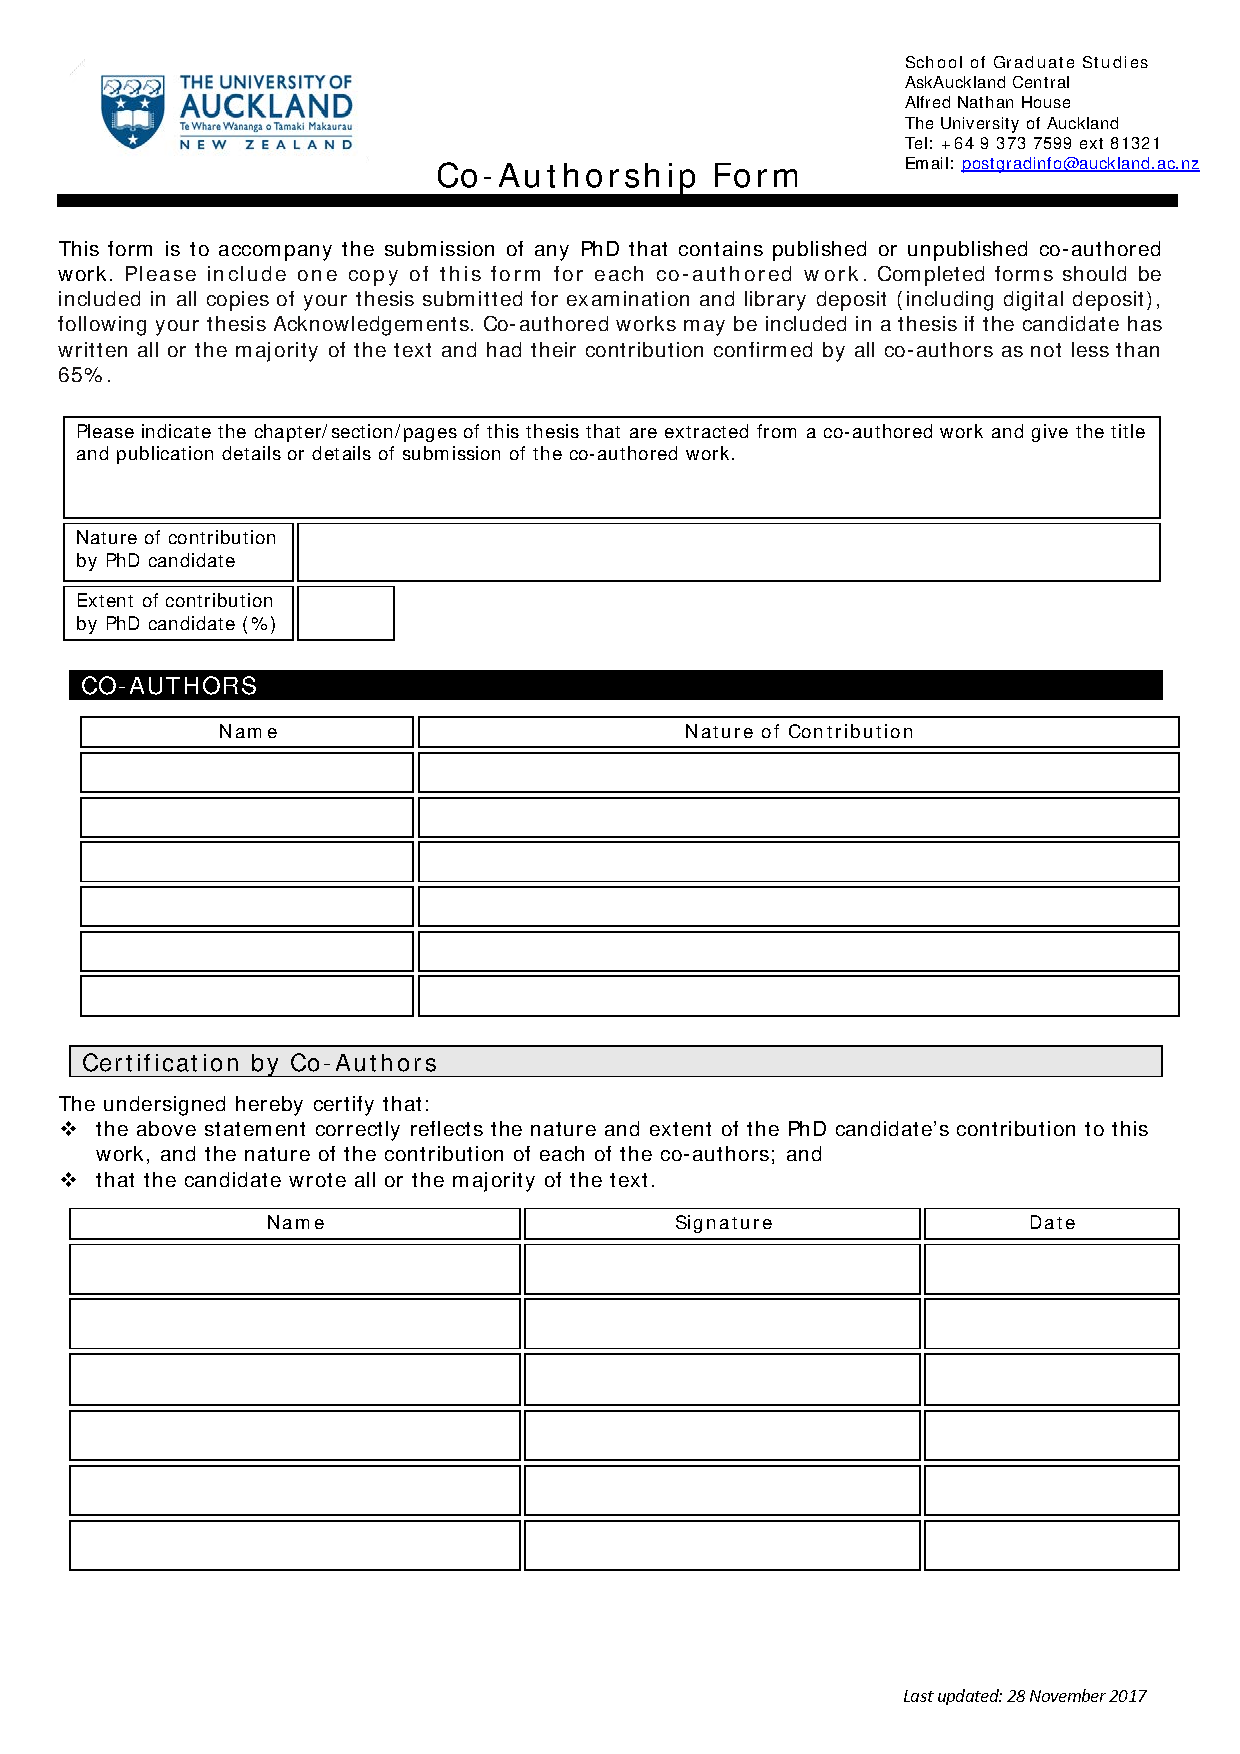
\includepdf[pages=-, openright=true, noautoscale=true, scale=0.9, pagecommand={}]{FrontBackmatter/co-authorship-form.pdf}
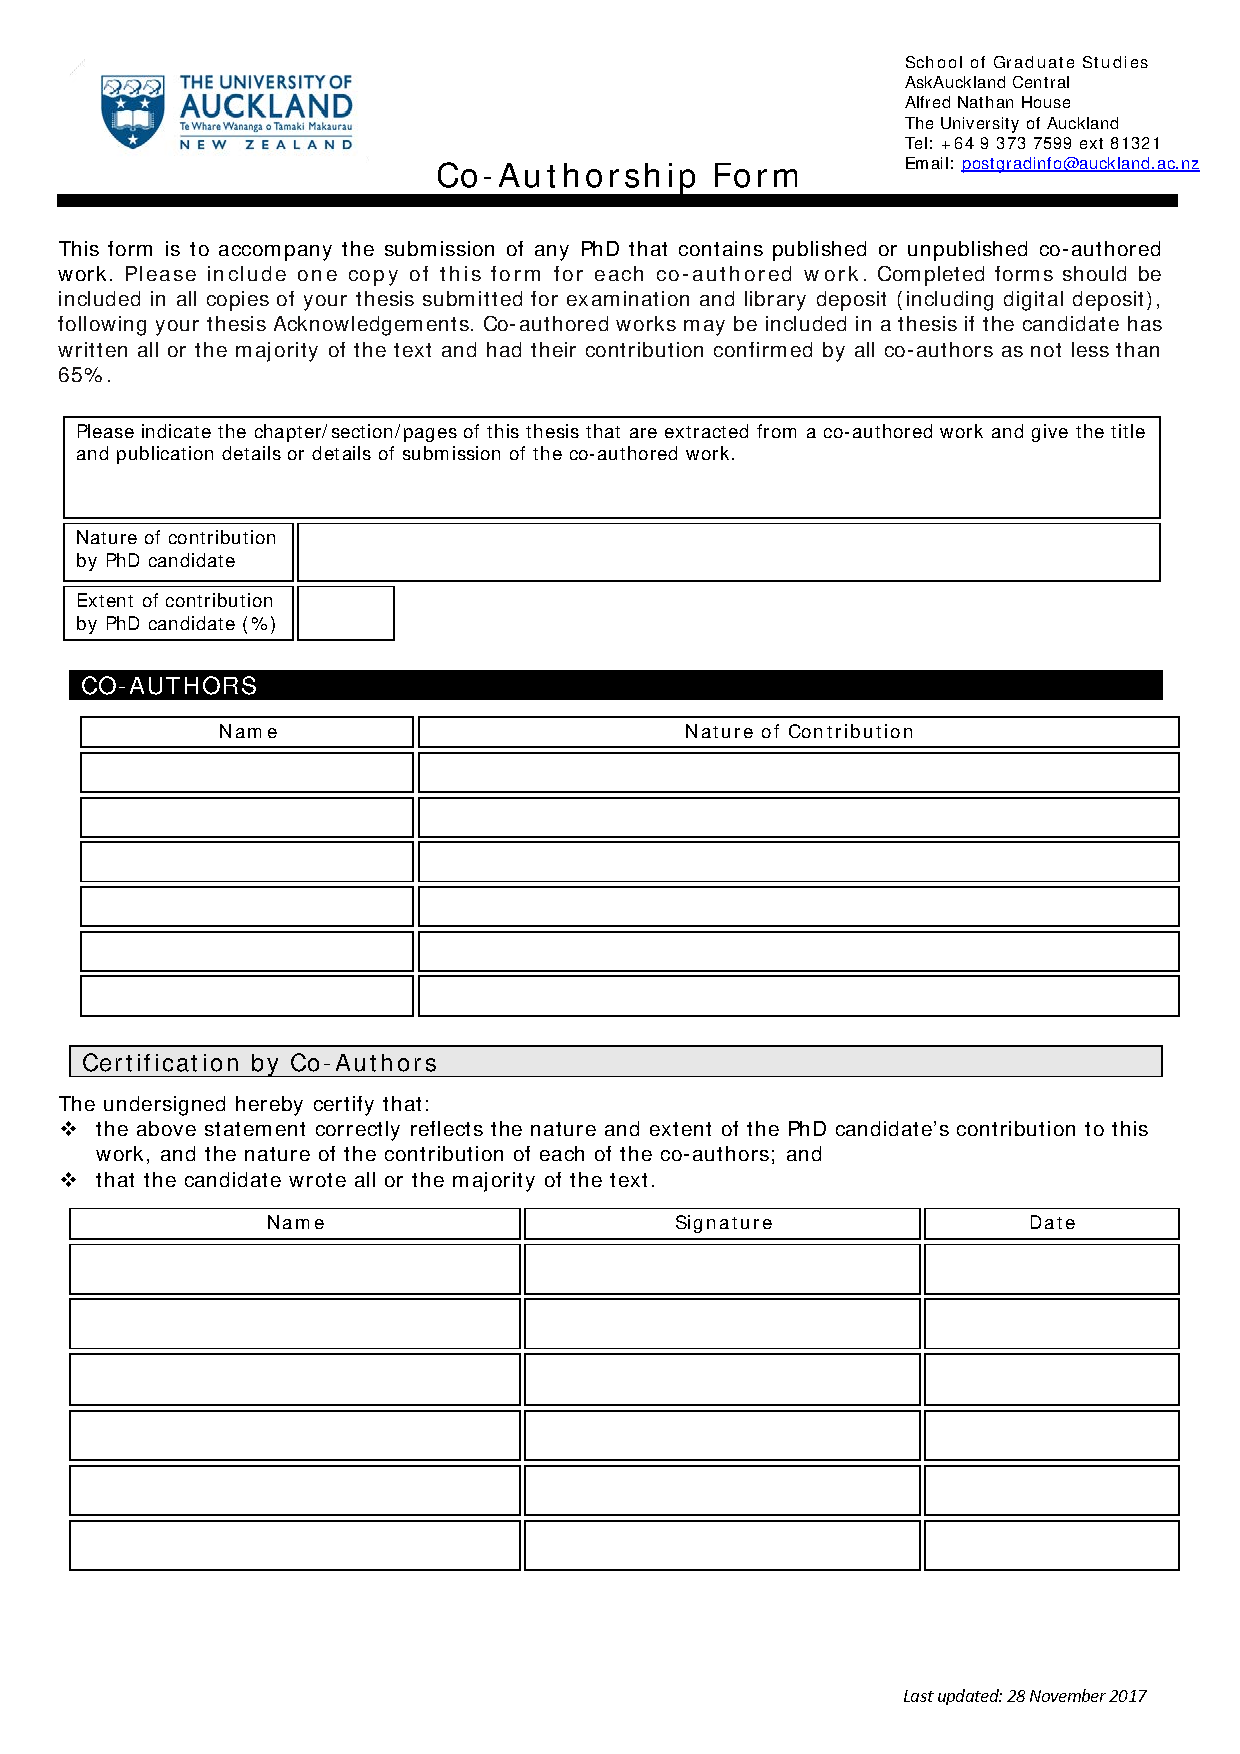
\includepdf[pages=-, openright=true, noautoscale=true, scale=0.9, pagecommand={}]{FrontBackmatter/co-authorship-form.pdf}
%\cleardoublepage%*******************************************************
% Acknowledgments
%*******************************************************
\pdfbookmark[1]{Co-Authorship Forms}{coauthorship}

%\begin{flushright}{\slshape
%    We have seen that computer programming is an art, \\
%    because it applies accumulated knowledge to the world, \\
%    because it requires skill and ingenuity, and especially \\
%    because it produces objects of beauty.} \\ \medskip
%    --- \defcitealias{knuth:1974}{Donald E. Knuth}\citetalias{knuth:1974} \citep{knuth:1974}
%\end{flushright}
%
%

\bigskip

\begingroup
\let\clearpage\relax
\let\cleardoublepage\relax
\let\cleardoublepage\relax
\chapter*{Co-Authorship}
%Put your acknowledgments here.
%
%Many thanks to everybody who already sent me a postcard!
%
%Regarding the typography and other help, many thanks go to Marco
%Kuhlmann, Philipp Lehman, Lothar Schlesier, Jim Young, Lorenzo
%Pantieri and Enrico Gregorio\footnote{Members of GuIT (Gruppo
%Italiano Utilizzatori di \TeX\ e \LaTeX )}, J\"org Sommer,
%Joachim K\"ostler, Daniel Gottschlag, Denis Aydin, Paride
%Legovini, Steffen Prochnow, Nicolas Repp, Hinrich Harms,
%Roland Winkler, Jörg Weber, Henri Menke, Claus Lahiri,
%Clemens Niederberger, Stefano Bragaglia, Jörn Hees,
%Scott Lowe, Dave Howcroft, Jos\'e M. Alcaide, David Carlisle,
%Ulrike Fischer, Hugues de Lassus, Csaba Hajdu, Dave Howcroft, 
%and the whole \LaTeX-community for support, ideas and
%some great software.
%
%\bigskip
%
%\noindent\emph{Regarding \mLyX}: The \mLyX\ port was intially done by
%\emph{Nicholas Mariette} in March 2009 and continued by
%\emph{Ivo Pletikosi\'c} in 2011. Thank you very much for your
%work and for the contributions to the original style.
%

\endgroup

\cleardoublepage%*******************************************************
% Publications
%*******************************************************
\pdfbookmark[1]{Publications}{publications}
\chapter*{Publications}%\graffito{This is just an early --~and currently ugly~-- test!}
%This might come in handy for PhD theses: some ideas and figures have appeared previously in the following publications:

%\noindent Put your publications from the thesis here. The packages \texttt{multibib} or \texttt{bibtopic} etc. can be used to handle multiple different bibliographies in your document.

\begin{refsection}[ownpubs]
    \small
    \nocite{*} % is local to to the enclosing refsection
    \printbibliography[heading=none]
%\begin{thebibliography}{1}
%	\bibitem{wikibook}
%		\bibTitle{Manually Managing References}, 
%		\url{https://en.wikibooks.org/wiki/LaTeX/Manually_Managing_References};
%		2016
%	\bibitem{wombat2016}
%		Walther Wombat and Klaus Koala,
%		\bibTitle{The true meaning of 42} in: Journal of modern skepticism;
%		2016
%	\bibitem{lion2010}
%		Laura Lion, Gabrielle Giraffe and Carl Capybara,
%		\bibTitle{The dangers of asking the wrong question}, publishing house;
%		2010
%\end{thebibliography}
 
        
\end{refsection}



\cleardoublepage%*******************************************************
% Table of Contents
%*******************************************************
\pagestyle{scrheadings}
%\phantomsection
\pdfbookmark[1]{\contentsname}{tableofcontents}
\setcounter{tocdepth}{2} % <-- 2 includes up to subsections in the ToC
\setcounter{secnumdepth}{3} % <-- 3 numbers up to subsubsections
\manualmark
\markboth{\spacedlowsmallcaps{\contentsname}}{\spacedlowsmallcaps{\contentsname}}
\tableofcontents
\automark[section]{chapter}
\renewcommand{\chaptermark}[1]{\markboth{\spacedlowsmallcaps{#1}}{\spacedlowsmallcaps{#1}}}
\renewcommand{\sectionmark}[1]{\markright{\textsc{\thesection}\enspace\spacedlowsmallcaps{#1}}}
%*******************************************************
% List of Figures and of the Tables
%*******************************************************
\clearpage
% \pagestyle{empty} % Uncomment this line if your lists should not have any headlines with section name and page number
\begingroup
    \let\clearpage\relax
    \let\cleardoublepage\relax
    %*******************************************************
    % List of Figures
    %*******************************************************
    %\phantomsection
    %\addcontentsline{toc}{chapter}{\listfigurename}
    \pdfbookmark[1]{\listfigurename}{lof}
    \listoffigures

    \vspace{8ex}

    %*******************************************************
    % List of Tables
    %*******************************************************
    %\phantomsection
    %\addcontentsline{toc}{chapter}{\listtablename}
    \pdfbookmark[1]{\listtablename}{lot}
    \listoftables

    \vspace{8ex}
    % \newpage

    %*******************************************************
    % List of Listings
    %*******************************************************
    %\phantomsection
    %\addcontentsline{toc}{chapter}{\lstlistlistingname}
    \pdfbookmark[1]{\lstlistlistingname}{lol}
    \lstlistoflistings

    \vspace{8ex}

%	%    %*******************************************************
%	% Acronyms
%	%*******************************************************
%	%\phantomsection
%	\pdfbookmark[1]{Acronyms}{acronyms}
%	\markboth{\spacedlowsmallcaps{Acronyms}}{\spacedlowsmallcaps{Acronyms}}
%	\chapter*{Acronyms}
%	\begin{acronym}[UMLX]
%		\acro{CPG}{Central Pattern Generator}
%		\acro{DE}{Differential Equation}
%		\acro{ML}{Machine Learning}
%		\acro{QRoSE{Quarter-Robotic Soft Esophagus}
%		\acro{RCT}{Randomized Controlled Trials}
%		\acro{ROM}{Reduced-Order Modeling}
%		\acro{RoSE{Robotic Soft Esophagus}
%		\acro{SEMS}{Self-Expandable Metallic Stent}	
%	\end{acronym}
		 %*******************************************************
		% Acronyms
		%*******************************************************
		%\phantomsection
		\pdfbookmark[1]{Acronyms}{acronyms}
		\markboth{\spacedlowsmallcaps{Acronyms}}{\spacedlowsmallcaps{Acronyms}}
		\chapter*{Acronyms}
		\begin{acronym}[UMLX]
			\acro{AC}{Abdominal Compression}
			\acro{ASR}{Automatic Symbolic Regression}
			\acro{BIBPS}{Baseline of Intra-Bolus Presssure Signature}
			
			\acro{CAD}{Computer-Aided Design}
			\acro{CeG}{CNT embroidered Graphane}
			\acro{CNT}{Carbon Nanotube}
			\acro{CPG}{Central Pattern Generator}
			\acro{DE}{Differential Equations}
			
			\acro{EC}{Esophageal Cancer}
			\acro{FEM}{Finite Element Modeling}
			
			\acro{GPN}{Graphene Porous Network}
			\acro{HRM}{High Resolution Manometry}

			\acro{IBPS}{Intra-Bolus Presssure Signature}
			\acro{ILPS}{Intraluminal Presssure Signature}
			\acro{IW}{Indentation Wave}
			
			\acro{MIBPS}{Maximum of Intra-Bolus Presssure Signature}
			\acro{ML}{Machine Learning}
			
			\acro{PDMS}{Liquid Polydimethylsiloxane}
			\acro{PILPS}{Peak of Intraluminal Presssure Signature}
			\acro{PP}{Primary Peristalsis}
			\acro{PPW}{Primary Peristaltic Wave}
			\acro{QRoSE}{Quarter-Robotic Soft Esophagus}
			
			\acro{RCT}{Randomized Controlled Trials}
			\acro{RF}{Radial Force}
			\acro{ROM}{Reduced-Order Modeling}
			\acro{RoSE}{Robotic Soft Esophagus}
			\acro{ROT}{Region of Transition}
				
			\acro{SEMS}{Self-Expandable Metallic Stent}	
			\acro{SI}{System Identification}
			\acro{SL}{Supervised Learning}
			\acro{SNT}{Silver Nanotubes}
			\acro{SP}{Secondary Peristalsis}
			\acro{SPW}{Secondary Peristaltic Wave}
			\acro{UL}{Unsupervised Learning}
			
		\end{acronym}	
	\endgroup



%********************************************************************
% Mainmatter
%*******************************************************
\cleardoublepage
\pagestyle{scrheadings}
\pagenumbering{arabic}
%\setcounter{page}{90}
% use \cleardoublepage here to avoid problems with pdfbookmark
\cleardoublepage
\ctparttext{
``Thereafter rose Desire in the beginning, Desire, the primal seed and germ of Spirit.
Sages who searched with their heart's thought discovered the existent's kinship in the non-existent.''
\begin{flushright}
--\textbf{Rig Veda:10.129.4}\\
\end{flushright}

}
\part{The Motivation}

%************************************************
\chapter{Introduction}\label{ch:introduction}
%************************************************
%\section{Introduction} \label{intro:intro}


\section{Biologically-Inspired Soft Robotics}

Softness and compliance are two notable features that make humans
and animals capable of interacting efficiently in a complex environment.
Thus, in the field of robotics, understanding biological processes
and systems have always been a great source of inspiration for engineers
to develop more capable robots. Even though traditional robots
are well-read and investigated, they are as yet unable to adequately
fulfill the requirements of the interactions needed in variable and
unpredictable working states.

Although the capabilities of the traditional-bodied robots have seen
a lot of significant development, the demand for studying various
biological processes and developing systems which are capable of
soft and continuous interaction with the environment has led many
researchers to open the gateway of a new field of research known as
the soft robotics \citep{rus2015}. In the previous couple of years, the area of soft
robotics has progressed toward becoming a very much characterized
discipline with working practices.

Soft robotics is an area where the robots are designed by using soft
and compliant modules. The advantage of soft robots over rigid body
counterparts are involving infinite degrees of freedom and different
movements \citep{Yap2016}. Robots which can completely mimic various biological
process can be developed by combining multiple functional units
strategically to act as a single unit, which generates smooth actions
and adaptability to different environmental conditions. Some of the
advantages of soft robots are continuous body motion, large-scale
deformation, safe human-robot cooperation, minimal effort production
\citep{Katzschmann2016,Argiolas2016}, and basic manufacture with negligible coordination \citep{Argiolas2016}.

In rigid body control, the locomotion of which can be described by
six degrees of freedom but in soft-bodied robots, the movement cannot
be limited to planar motions. Due to the bending, buckling, wrinkling,
stretching, twisting, compressing, etc. nature of the soft materials,
developing a control system for such robots are very challenging. Controlling
soft robots demand new lines of modelling, control, dynamics
and advanced level planning \citep{rus2015}. One of the important aspects of
controlling bio-inspired soft robots is that all the parts of the robot
continuously interact and inspire each other. Despite the fact that a particular accord on these principles is developing in the soft robotics and
its related societies, the young field of bio-inspired soft robotics still
wants a robust and steady base like control theory for rigid robotics \citep{Pfeifer2007}. The theory needs to be further developed, and a substantial amount
of work toward a better understanding of how the behaviour of the
robot is influenced by its underlying governing dynamics rather than
controlled is still needed to be achieved \citep{Pfeifer2012}. To have a grasp of the
science, researchers are performing an exhaustive number of different
experiments on the soft robots which result in the collection of
extensive experimental data.

\section{Machine Learning Modelling and Control in Soft Robotics}

\ac{ML} as an arrangement of strategies that can naturally
distinguish patterns in data, and afterwards utilise the revealed
patterns to foresee future data or to perform different sorts of decision
making under vulnerability. Use of \ac{ML} strategies to
massive databases is called as data mining \citep{Alpaydin2020}. However, it should be
noted that even when one has an evidently large dataset, the effective
number of data points for particular cases of interest might be quite
small. In fact, data from a variety of spaces shows a property known
as the long tail, which implies that a couple of things are exceptionally
similar. However, most things are very uncommon. For instance,
twenty percent of Google hunts every day have never been seen \citep{Murphy2012}.
This implies the centre measurable issues concerning generalising
from small examples sizes, are still exceptionally pertinent even in the
era of big data.

\section{Biological Swallowing and Endoprosthetic Stenting}

Swallowing is a complex but orderly physiological process transporting
saliva or food from the mouth to the stomach, aided by peristaltic
contractions of the esophageal wall, generated by \ac{CPG} \citep{Jean2001}. Any esophageal impairment compromises the
efficiency of swallowing, is known as dysphagia. Severe pathologies,
for instance, benign esophageal strictures from various injuries,
\ac{EC}, and esophageal perforations, distressing lumen patency
explicitly leading to dysphagia \citep{Garcia2010}. Unaccompanied by
comprehensive care, a vicious cycle materializes as malnutrition and
dehydration aggravating the dysphagia itself, subsequently increasing
morbidity and even mortality.

A silicone covered \ac{SEMS} is a tubular
braided mesh of interwoven helical springs made of corrosionresistant
materials, like nitinol, stainless steel, and polymers. Malignant
and benign esophageal strictures from \ac{EC}, can be
addressed with the endoprosthetic stent placement, commonly known
as esophageal stenting \citep{hanawa2009materials}. These stents are proven to be efficient endoprosthetic
management for both malignant and benign esophageal
strictures, as they could hold open the esophagus and hence, relieve
the impediments of compromised lumen patency in such cases \citep{hirdes2013vitro}.

However, this method of palliative treatment does have its inadequacies,
and one of the significant shortcomings is stent migration,
which is the movement of the implanted stent from its initial position,
caused due to the stent interaction with the continuous peristaltic
contractile forces of the esophageal wall \citep{sharma2010role}. Stent radial force (RF), force applied by the stent on the esophageal lumen, is a crucial design parameter of a stent for maintaining the in situ lumen patency, which is, unfortunately, still an unknown parameter due to the poorly understood association of the RF and clinical outcomes. The efforts to mitigate
migration, to improve stent removability and flexibility, and to ensure
stent patency have revolutionized the stent designs. To study stent
inadequacies for improving stent design, conventional techniques like
manometry and videofluoroscopy on the patients are less preferred
because the techniques are not very comforting for the patients, and
there are major ethical concerns associated with such kind of studies.
Thus, evidence to show which stent design is better than the other is
confined to a few \ac{RCT} in patients with
malignant esophageal strictures \citep{hirdes2013vitro}.

\section{Robotic Soft Esophagus}

The current research is an augmentation of a research program that
explores biomimetic esophageal swallowing. A \ac{RoSE} has been developed as an alternative platform for mimicking
the human swallowing process under different rheological and
medical conditions (\autoref{fig1_RoSE_f1}) \cite{Dirven2014}. The capability of \ac{RoSE} is to generate
peristaltic waves of different characteristics similar to the waves
generated when food bolus travels from upper to the lower esophagus
in humans.

\begin{figure}[bth]
	\myfloatalign
	{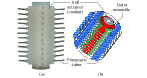
\includegraphics[width=\linewidth]{images/Ch1/fig1_RoSE_f1}} \quad
	\caption[Robotic Soft Esophagus (RoSE)]{Robotic Soft Esophagus (RoSE). (a) RoSE actuator (conduit), and (b) isometric view of \ac{CAD} assembly of RoSE.}\label{fig1_RoSE_f1}
\end{figure}

\ac{RoSE} is made up of Ecoflex 00-30 (Smooth-On, USA), which is a soft
and highly stretchable platinum-catalyzed silicon rubber. The physical
dimension of \ac{RoSE} matches the attributes of the human esophagus
\cite{Dirven2014}. \ac{RoSE} has twelve equally spaced layers, and in each layer, four
pneumatic chambers are present surrounding the conduit. The purpose
of these air chambers is to deform sequentially layer by layer
under the supplied air pressure in such a way that the shape of the
deformation can take the form of a traveling peristaltic wave from
the top layer to the bottom layer \cite{Dirven2015}. \ac{RoSE} is a true example of a
robot mimicking a biological process, and performing tests on such a
robot instead of a human being can save the researchers from ethical
concerns and accessibility time, and it can widen the range of different
measurements and evaluation schemes \cite{Dirven2015}.


\section{Research Motivation}

There are two reserach motivation for this study. The first motivation of
this research is to validate \ac{RoSE} as a novel in vitro platform to perform
a wide-ranging assessment of stent-behavior. The second motivation
of this research is to set out on another convention: establishing and
implementing \ac{ML} techniques as the first and foremost
above traditional analysis.

\subsection{Motivation 1}

Testing bolus formulation and transport, stent behavior assessment,
and swallow efficacy with clinical trials are hindered by the interperson
swallow and the inter-swallow variability in human test subjects.
Besides, due to the less known relationship between the mechanical
properties of the esophageal stents and their clinical outcome, the
stenting guidelines are still poorly defined. Further, evidence from the
\ac{RCT} that can be used to test the clinical performance of the stent is
limited.
In the mathematical field, very few numerical models have examined
the interaction between the stent and the esophagus under peristalsis.
Additionally, it is challenging to model the complex shear fields generated
by peristaltic actuation and their associated time-shear dependent
behavior.
Soft robotics in vitro models such as \ac{RoSE} has proved to be a complementary
and supplemental approach to mathematical models, and
clinical studies to investigate the human physiology and to validate
medical procedures. Since \ac{RoSE} can physically mimic the human swallowing
behavior; thus, instead of actual patients, it can be used to
conduct the study on various stent designs, and their inadequacies
and effect on swallow efficacy, before implanting them in patients
with malignant and benign esophageal strictures (\autoref{fig2_funnel}).

\begin{figure}[bth]
	\myfloatalign
	{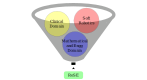
\includegraphics[width=\linewidth]{images/Ch1/fig2_funnel}} \quad
	\caption[Relationship between RoSE and different research domains.]{Relationship between RoSE and different research domains. \ac{RoSE} combines and integrates the concepts from four research domains: clinical, mathematical, engineering, and soft robotics}\label{fig2_funnel}
\end{figure}

\subsection{Motivation 2}

Conventional methods for discovering the partial \ac{DE}
of a system are rooted in laws of physics, conservation laws,
and phenomenological behavior. In any case, there remain numerous
complex systems like \ac{RoSE} that have escaped quantitative investigative
depictions or even characterization of an appropriate selection of
variables.
Currently, \ac{RoSE} does not have any dynamic equation to describe its
actuation principles or its physics. Finding out its governing \ac{DE} will not only help in better understanding its physics,
but it will also contribute to design a better adaptive close loop control
strategy for the robot, which can control the bolus transit behavior
by receiving feedback from the displacement sensors located on the
surface of the conduit. Instead of designing a black-box model of the
robot for control, a grey box model can be implemented, if some of
the dynamics of the robot are known.
In addition, a large number of different types of experiments with
manometry, videofluoroscopy, articulography, and motion capture
have already been performed on the robot resulting in the collection of
an extensive amount of datasets. Discovering the \ac{DE} from the collected datasets will give relevance to it as well as
meaning to the accomplished experiments.

\section{Aim and Objectives}

This study has two key aims. Firstly, the aim is to validate the application of \ac{RoSE} in performing a wide-ranging assessment of stent-related measurements and behavior for substantial equivalence. Secondly, the aim is to actuate the \ac{RoSE} conduit with pre-defined peristaltic wave trajectories by data-driven ML-based modeling and control. While the former aim, addresses the question of usability of \ac{RoSE} in the area of endoprosthetic stent testing, the later offers a novel approach to model and control \ac{RoSE} for understanding its underlying dynamics.  Objectives 1, 2, and 3, 4 will contribute to the fulfillment of the first and second aims, respectively.  With the accomplishment of the primary aim, \ac{RoSE} can emerge as a powerful in vitro platform for the endoscopic industries and clinicians to test their new stent designs in terms of migration and the occurrence of any kind of dysfunctionality during and after the stent implantation. The completion of the second aim will enhance this capability of \ac{RoSE} further. 

\subsection{Objective 1: RoSE Capability in Investigating Stent Radial Force and Migration.}

The objective assesses the effect of stent \ac{RF} on the migration of stents in the \ac{RoSE} conduit, which occurs due to repeated peristaltic contractions. The presented results can validate \ac{RoSE} as a novel platform to assess various stent behaviors, which can help the researchers and the endoscopists to elucidate the patency of the stents in the occurrence of unfavorable events, during and after the stent implantation. The objective was achieved by completing the following subtasks (\autoref{fig3_Obj1}):

\begin{figure}[bth]
	\myfloatalign
	{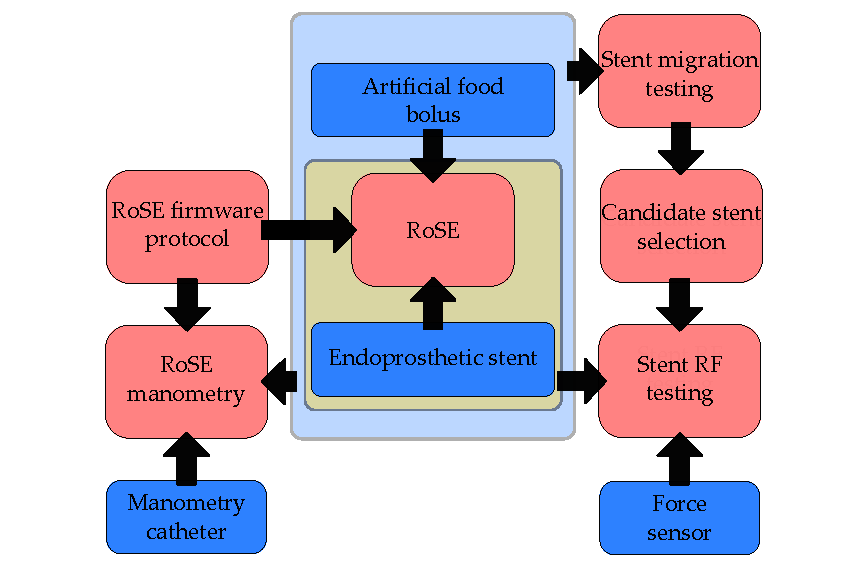
\includegraphics[width=\linewidth]{images/Ch1/fig3_Obj1}} \quad
	\caption[Sequence of the conducted subtasks to achieve objective 1 and 2.]{Sequence of the conducted subtasks to achieve objective 1 and 2.}\label{fig3_Obj1}
\end{figure}

\begin{itemize}
	\item Literature review
	
	Validating the capability of \ac{RoSE} in the area of stent testing requires reviewing relevant literature which underlines the major stent designing parameters and their effect on the stent performance. State of the art incorporating various topics on clinical studies on stent implantation, mathematical stent modeling, stent \ac{FEM}, and stent in vitro testing are studied for the attainment of the objective.  Besides, a thorough literature review on swallowing, \ac{EC}, and dysphagia is also conducted. 
	
	\item Development of RoSE firmware protocol
	
	Custom firmware modules, written in Python 3.7, are developed on Raspberry Pi 3B+ to assert the robot, with independent, continuously variable, pressure input. The \ac{RoSE} firmware protocol is divided into two significant sub-modules for stent \ac{RF}, and migration and bolus swallow efficacy testing. While, the first sub-module deals with simultaneous inflation and deflation of the \ac{RoSE} conduit, the second one generates peristaltic waves in \ac{RoSE}.
	
	\item Designing stent deployment framework
	
	A deployment framework following the endoscopists approach to deploying stents in the human esophagus was developed and employed throughout this study. 
	
	\item Artificial food bolus formulation
	
	Food boluses of varying consistencies were prepared in the laboratory using a commercial food thickener, specially formulated for dysphagia patients. The consistencies were quantified by evaluating the viscosity using a viscometer.
	
	\item Stent migration testing
	
	Five commercial, covered \ac{SEMS}s having distinct structures, cover materials, and cover material patterns, and similar dimensions were initially tested for stent migration in \ac{RoSE} with and without food bolus. Based on the maximum and minimum recorded migration,  candidate stents were selected for further measurement and analysis of different stent-related parameters.
	
	\item Force Sensor testing for RF measurement
	
	\item Stent RF testing
	
	By contracting and expanding the \ac{RoSE} conduit, stent \ac{RF} testing was performed. The testing protocol consists of repeatedly measuring the \ac{RF} applied by the stent on the conduit wall during its loading and unloading to evaluate its migration behavior. 
\end{itemize}

\subsection{Objective 2: RoSE In Vitro Platform for Studying the Impact of Stent Implantation on Bolus Swallow Efficacy.}

The objective is to examine the impact of the stent deployment on the \ac{RoSE} bolus swallow efficacy. Besides, it also includes analyzing the effect of stent dysfunctionality on bolus transport, and hence, swallow efficacy. \ac{RoSE} manometry investigation presents evidence that extends the knowledge of swallow efficacy after stent implantation during dysphagia (\autoref{fig3_Obj1}). 

\begin{itemize}
	\item Manometry setup and calibration
	
	A manometry setup consisting of a catheter (long flexible tube) and a data acquisition system was calibrated before installing the catheter into the \ac{RoSE} conduit due to the inaccessibility and unavailability of suitable instruments for in situ calibration. The catheter was positioned akin to the clinical in vivo observations.  
	
	\item RoSE manometry testing
	
	The methodology of \ac{RoSE} manometry testing can be distributed into two steps. In the first step, experiments and investigation for a regular stent operation were conducted, then in the second step, study for stent dysfunctionality was carried out. The investigation used both qualitative and quantitative analysis in order to gain insights into the effect of \ac{RoSE} swallow efficacy with implantation of stents. 
\end{itemize}
\subsection{Objective 3: Sparse Data-Driven Discovery of RoSE Dynamic Differential Equations}

The third objective is to discover the underlying dynamic \ac{DE} of \ac{RoSE}
by applying data-driven ML techniques. The \ac{DE} captures the \ac{RoSE}
peristaltic conduit deformation with respect to the applied pressure at
any instant of time. In contrast to previous \ac{RoSE} models, the \ac{DE} model
is dynamical in nature and solely depends on the captured data. The
model enhances the understanding of the kinematic and dynamic
features of \ac{RoSE}. The following tasks were undertaken to achieve this
objective (\autoref{fig4_Obj3}):

\begin{figure}[bth]
	\myfloatalign
	{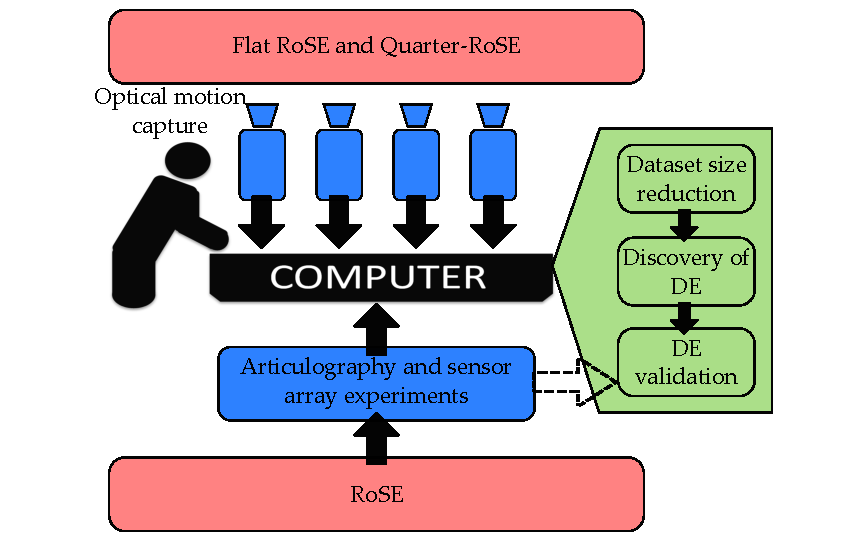
\includegraphics[width=\linewidth]{images/Ch1/fig4_Obj3}} \quad
	\caption[Sequence of the conducted subtasks to achieve objective 3.]{Sequence of the conducted subtasks to achieve objective 3.}\label{fig4_Obj3}
\end{figure}

\begin{itemize}
	\item Literature review
	
	Literature from the areas of \ac{ROM}, ML,
	and soft robotics was reviewed to analyze the existing modeling
	strategies. Various ML techniques were explored, along with their
	working principle and limitations. Besides, a thorough literature
	review on swallowing and dysphagia were also conducted.
	
	\item Design of Quarter-RoSE
	
	\ac{RoSE} has limited visibility inside its conduit, which challenges the
	collection of the experimental data needed for the \ac{DE} discovery.
	To address this issue, a \ac{QRoSE}
	was developed to observe and model the occlusive motion of the
	conduit of \ac{RoSE}.
	
	\item Optical motion capture
	
	To capture \ac{QRoSE} conduit deformation data, a column of retroreflective
	markers were placed on the conduit. By using the Vicon
	optical motion capture system, time-series datasets were collected
	by tracking the movement of the markers.
	
	\item Dataset size reduction
	
	To reduce the computational complexity, \ac{ROM} techniques were
	applied to the size of the collected dataset.
	
	\item Discovery of RoSE DE
	
	A data-driven ML technique which promotes sparsity was applied
	on the reduced dataset to discover the \ac{DE} of \ac{RoSE}.
	
	\item Validation of the DE
	
	The conduit deformation calculated from the discovered \ac{DE} was
	validated by collecting data from articulography and stretchable
	displacement sensor array experiments.
\end{itemize}

\subsection{Objective 4: Design of Sparse Model-Based Predictive Controller}

\section{Scope}

The first part of the research was about validating the applicability of \ac{RoSE} in the area of stent design and testing that can help the researchers and the endoscopists to elucidate the patency of the stents in the occurrence of unfavorable events, during and after the stent implantation. To clarify the extent, the study remains within the following research criteria. 

\begin{itemize}
	
	\item Even though \ac{RoSE} mimics the esophagus in various physiological ways but its conduit still lacks artificial strictures. Thus, all the multiple stent testings were carried out in normal swallowing conditions of RoSE.  
	
	\item The investigation of the stent testing has not considered the distribution of different muscle fiber regions because the entire \ac{RoSE} conduit is made up of the same silicone rubber material (Ecoflex 0030, Smooth-on, USA).
	
	\item The study is strictly limited to proving the usability of \ac{RoSE} in stent testing. It does not focus on the various design aspects of the stents that were used for conducting this research.

\end{itemize}

The second part of the research was about finding novelty in the area of soft robotics by implementing \ac{ML}, and optimization techniques to model and control \ac{RoSE} under different bolus transit behavior. Therefore, it abides the following research criteria:

\begin{itemize}
	\item  The derivation of the \ac{DE} of \ac{RoSE} has not considered the variation in properties of the material used to design the robot. The assumption only discusses the current state of the material and neglect any change in its qualitative or quantitative characteristics over time and varying environmental conditions like pressure and temperature.
	
	\item Any given marker on the surface of the robot moves along pre-defined coordinates of the x, y, and z-axis. For this research, movement along the y and z-axis are considered.
	
	\item All the sensors implemented in this research are off-the-shelf since the performance of the earlier designed and fabricated sensors are not up to the desired level.   

\end{itemize}

\section{Research Contributions}


Investigating stent \ac{RF} has been a continuing concern within the clinicians and the scientific community. It has been challenging to fully predict the clinical outcome of a stent based on its \ac{RF}. However, the presented results show that \ac{RoSE} can provide a novel platform to evaluate the substantial equivalence of esophageal stents of different characteristics. Besides, the results can provide the researchers with a deep insight into the patency of the stents and bolus swallow efficacy in the esophagus after stent implantation. The findings can make an essential contribution to the field of stent designing and testing. 

The results comparing the efficiency of the stents could aid the endoscopists in the selection of a suitable stent for an individual patient, which is otherwise guided solely by their experience and availability of the stents. The results will also aid in the optimization of future stent designs to improve the behavior of the stent during deployment and to mitigate migration. 

The analysis of the bolus pressure signatures with stenting in \ac{RoSE} has extended the knowledge of swallow efficacy after stent implantation during dysphagia. The presented in vitro study adds to the growing body of research that considered esophageal peristalsis for stent-related measurements. To the extent of our knowledge, no prior research has done endoscopic manometry in the presence of stents.  Additionally, the study has been one of the first attempts to examine parametric studies correlating the effect of stent implantation, and dysfunctionality on swallow efficacy. 

Soft robotic techniques provide compliance and unique shapes
to robots. In contrast to the rigid-bodied robots, soft robots have an advantage of infinite degrees of freedom, which allows them to move freely and mimic various movement patterns of humans. However, when it comes to modeling and control, the advantage becomes a disadvantage because all the parts of the robot continuously interact and inspire each other.  This study makes several noteworthy contributions to the
area of soft robotics modeling. To the best of our knowledge, this is the first time that ML has been applied to identify a structural and
parametric dynamical model of \ac{RoSE}. The methods revealed
the underlying dynamics of the soft-bodied \ac{RoSE} in the form of
\ac{DE} model. In contrast to the earlier models of \ac{RoSE}, the
the model presented in this research is dynamical. Since ML solely depends on the captured data, the discussed methodology is not robot specific and does not depend upon the actuation system and morphology of the robot. The method undertaken in this study is general, while \ac{RoSE} is a case study. It can be extended to any soft-robotic system, provided an input-output dataset can be generated. The \ac{DE} discovered in this
study also explicitly define the nonlinear behavior of the robot.
The analysis of the \ac{DE} has extended our knowledge about the
deformation of the \ac{RoSE} conduit. 
%*****************************************
%*****************************************
%*****************************************
%*****************************************
%*****************************************



\ctparttext{''A person is said to be established in self-realization and is called a yogi when he is fully satisfied by virtue of acquired knowledge and realization. Such a person is situated in transcendence and is self-controlled. He sees everything—whether it be pebbles, stones or gold—as the same.''\\
\begin{flushright}
--\textbf{Bhagavad Gita:6.8}\\
\end{flushright}
}

\part{The Path of Knowledge}


\chapter{Literature Review}\label{ch:methodology}

\section{Medical Background of Esophageal Swallowing}

Swallowing is a complex but orderly physiological process transporting saliva or food from the mouth to the stomach. The swallowing physiology and anatomy are elucidated with the critical insights from the in vivo studies \citep{Dodds1989}. Any esophageal impairment compromises the efficiency of swallowing, is known as dysphagia \citep{Groher2015}. Severe pathologies, for instance, benign esophageal strictures from various injuries, esophageal cancer, and esophageal perforations, distressing lumen patency explicitly leading to dysphagia. Unaccompanied by comprehensive care, a vicious cycle materializes as malnutrition and dehydration aggravating the dysphagia itself, subsequently increasing morbidity and even mortality \citep{Garcia2010}. The standard clinical practices involve evaluation of the etiology of the swallowing deficit using perception studies, and in vivo analysis, followed by intervention strategies for nutritional support \citep{Kuo2012}. Depending upon the severity, the method of maintaining nutrition varies from oral dietary supplements, texture modified foods, implanting nasogastric feeding tubes, surgical correction, endoscopic dilation of the sphincters, and esophageal stenting \cite{Groher2015,Cichero2017}.

\subsection{Swallowing Process}
The anatomy of the human digestive system begins with munching, mashing, and mixing the food in the mouth and ends at the anus (\autoref{fig1_Dig_sys}). The process of swallowing, which is sometimes referred to as deglutition, involves transportation of food bolus from the oral cavity to the stomach through the esophagus with the aid of peristaltic waves in the esophageal conduit, generated by central pattern generators (CPGs). 
The desired result of swallowing is not only the successful transportation of food but also the removal of the food particles from the respiratory tract so that the respiratory tract does not ingest any unwanted particles. \cite{Miller1986,Miller1987,lang2009brain}. 

\begin{figure}[bth]
	\myfloatalign
	{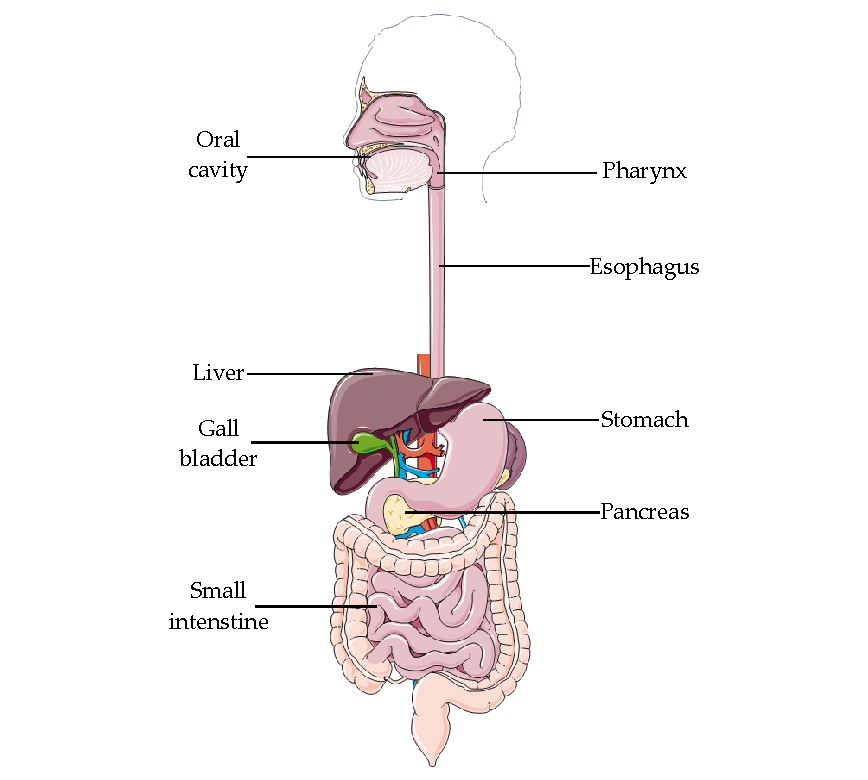
\includegraphics[width=\linewidth]{images/Ch2/fig1_Dig_sys}} \quad
	\caption[Anatomy of human digestive system.]{Anatomy of human digestive system.}\label{fig1_Dig_sys}
\end{figure}

\subsection{Stages of swallowing}
The neurophysiological control of the swallowing process comprises of three distinct phases where each phase is interacting with each other. The degree of dependence of each stage on the neuron control varies in each phase  \citep{lang2009brain}.

\subsubsection{Oral preparatory stage}
The oral preparatory phase is responsible for the primary preparation of the food bolus before the bolus enters the pharynx. After the mastication, it breaks down the ingested food in sufficiently small sizes and mixes it well with the saliva for transport through the pharynx and esophagus for digestion within the stomach \citep{Miller1986}.

\subsubsection{Pharyngeal stage}
The pharyngeal stage does the propelling of the food bolus to the esophagus. While doing the transport, it consistently coordinates with the respiratory tract so that it can be protected from the unwanted food particles. Four major activities done by the pharyngeal stage are \citep{Miller1986}. 

\begin{itemize}
	\item  Propelling the food bolus.
	\item  Inhibition of respiration
	\item  Closure of the palatopharyngeal isthmus
	\item  Constiction of the larynx    
\end{itemize}

\subsubsection{Esophageal stage}

The esophageal stage follows the pharyngeal stage, but it can function completely independent of any other stages of swallowing and has its own distinct neural control \cite{Miller1986, Miller1987, lang2009brain, Dodds1989}. The esophagus (Latin: \textit{oesophagus}), 180 to 260 mm in length, consists of a muscular tube that spans rostral caudally from the pharynx in the upper aspect, down to the stomach whose elementary function is to push the swallowed food and fluid from the oral cavity to the stomach by peristaltic contractions (\autoref{fig1_Dig_sys}) \cite{brasseur1987fluid,Miller1986,chen2009food}. 


\begin{figure}[bth]
	\myfloatalign
	{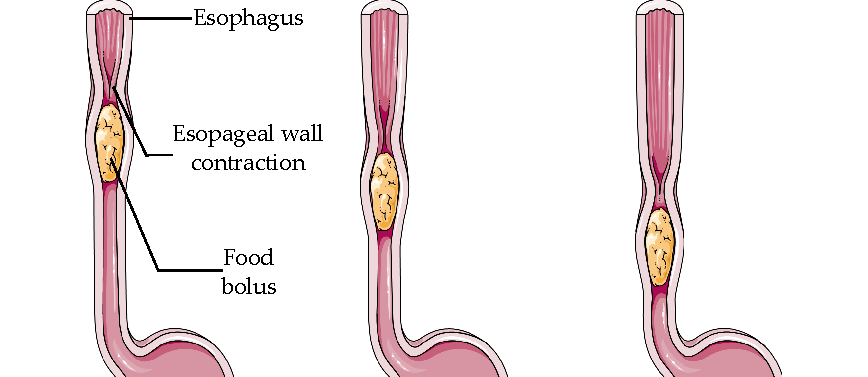
\includegraphics[width=\linewidth]{images/Ch2/fig2_Peristalsis}} \quad
	\caption[Esophageal peristalsis]{Esophageal peristalsis. The process of swallowing involves transportation of food bolus from the oral cavity to the stomach through the esophagus with the aid of esophageal wall contractions generated by spatio-temporal peristaltic waves.}\label{fig2_Peristalsis}
\end{figure}

\autoref{tab1_esophagus} summarizes all the relevant attributes of the human esophagus. The esophageal wall is made up of mucosa, submucosa and muscularis propria. The muscularis propria consists of outer longitudinal and inner circular muscle fibers, which activates sequentially to generate an esophageal wall contraction behind the bolus (\autoref{fig2_Peristalsis}) \cite{brasseur1987fluid,Miller1986,Miller1987,Dodds1989}. The fast movement of the bolus does not occur in the supine position, which evident the fact that bolus velocity is mostly governed by gravity \cite{mashimo2006physiology,brasseur1987fluid}. However, it has been shown that the process does not depend on gravity for
transport, as swallowing can be conducted in an inverted person \cite{chen2009food}. 

\begin{table}
	\myfloatalign
		\caption[Attributes of human esophagus and esophageal peristaltic transport.]{Attributes of human esophagus and esophageal peristaltic transport.}  \label{tab1_esophagus}
	\begin{tabularx}{\textwidth}{Xl} \toprule
		\tableheadline{Esophagus quantitative attributes}\\
		\midrule
		\tableheadline{Attribute} & \tableheadline{Magnitude} \\ \midrule
		Esophagus conduit length & 180 - 260 mm  \cite{brasseur1987fluid,Dodds1989}\\
		Conduit diameter & 20 - 23 mm \\
		Peristalsis wave velocity & 20 - 40 mms$^{-1}$  \cite{brasseur1987fluid,Jean2001}\\
		Wavefront length & 30 - 60 mm \\
		Wave seal pressure & 15 KPa  \cite{brasseur1987fluid}\\
		\midrule
		\tableheadline{Esophagus qualitative attributes}\\
		\midrule
		\tableheadline{Attribute} & \tableheadline{Behavior} \\ \midrule
		Wall material composition &  \multirow{2}{*}{\begin{tabular}[c]{@{}l@{}}Mucosa, submucosa,\\ and muscularis propria \citep{mashimo2006physiology}\end{tabular}} \\
		& \\
		Wall material feature & Compliant, and continuous\\
		Muscle fiber type & Longitudnal, and circular  \citep{mashimo2006physiology}\\
		Muscle distribution & Striated, and smooth \citep{mashimo2006physiology}\\
		Transport type & Peristaltic \cite{ghosh2006physiology}\\
		Wave shape & Sinusoidal  \\
		\midrule
		\tableheadline{Peristalsis attributes} \cite{ghosh2006physiology, Dodds1989, lang2009brain}\\
		\midrule
		Peristalsis type & Primary, and secondary\\
		Primary peristalsis (\ac{PP}) location & Smooth, and striated\\
		Primary peristalsis mechanism & Central\\
		Secondary peristalsis (\ac {SP}) location & Elicited from incomplete \ac{PP}\\
		
		\bottomrule
	\end{tabularx}

\end{table}

\subsubsection{Swallowing Mechanism}


Videofluoroscopy, and manometry techniques are used hand in hand to determine the \ac{ILPS}. In an esophageal peristaltic transport of food bolus, the manometry and videofluoroscopic recordings can be distributed into two \ac{ILPS} segments (\autoref{fig4_BolusPressureSig}) \cite{brasseur1987fluid,ren1993determinants,ghosh2006physiology}. In the first segment, within the bolus fluid, the recorded pressure is solely due to the hydrodynamic bolus pressure, which is also known as the \ac{IBPS}. At the tip of the bolus tail, the pressure undergoes a transition from \ac{IBPS} to esophageal direct contact pressure with the manometry catheter, which can be regarded as the second segment. The contact pressure is the \ac{PILPS}, which reflects the maximum esophageal muscle squeeze pressure aboove the bolus tail \citep{ghosh2006physiology}. The \ac{MIBPS} occurs at the bolus tail tip, and after which, no bolus fluid exists, leading to direct contact pressure. Since pressure cannot be transmitted axially in the absence of bolus fluid; thus, these two segments are independent of each other \cite{brasseur1987fluid}.  

\begin{figure}[bth]
	\myfloatalign
	{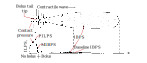
\includegraphics[width=\linewidth]{images/Ch2/fig4_BolusPressureSig}} \quad
	\caption[Schematic of axial distribution of intraluminal pressure signature  (ILPS) in an esophagus.]{Schematic of axial distribution of Intraluminal Pressure Signature  (ILPS) in an esophagus \cite{brasseur1987fluid}.}\label{fig4_BolusPressureSig}
\end{figure}

A dry swallow is an act of swallowing something without the aid of any liquid like water. It is associated with the swallowing of the air bolus. As there is no bolus present, hence there is no distension on the muscle of the esophagus, which results in the generation of low \ac{PILPS} waves \cite{hollis1975effect}. Wet swallows associated with liquid bolus of lower volume (<1 ml) have exhibited lower \ac{PILPS}, similar to dry swallows. However, wet swallows of bolus volume greater than 2 ml, have shown higher \ac{PILPS}, slower wave speed, and greater contraction wave duration as compared to low volume bolus. Besides, the strength of the esophageal contractions depicted by \ac{PILPS}, remains the same for all bolus volume higher than 2 ml, which indicates the fact that a critical bolus volume is required to initiate \ac{PP}. Additionally, \ac{PILPS} of the contraction waves and other parameters cannot be consciunsupersly altered \cite{hollis1975effect}. 

The \ac{IBPS} remains almost equal throughout the length of the esophagus but, \ac{IBPS} increases with bolus volume and bolus viscosity. Additionally, the dependence of \ac{IBPS} on bolus viscosity is only significant for bolus volume above 10 ml. Similarly, bolus transit time also does not vary throughout the esophagus, and it is independent of bolus volume and viscosity. 

A successful transit of the bolus is referred to as effective
peristalsis while, ineffective peristalsis is often associated with
the residue of food particles left in the esophagus \citep{ghosh2006physiology}. In an effective bolus transport, maximum intraluminal cross-sectional diameter generally increases as the bolus moves distally. While, increase in bolus volume significantly increases the diameter, the increase in viscosity have not shown any significant impact on it \cite{ren1993determinants}. For an ineffective peristalsis, when the esophageal muscular contractions are not enough to occlude the esophagus, the magnitude of \ac{MIBPS} remains closer to \ac{PILPS}. For a succesful bolus transport, \ac{PILPS}-\ac{BIBPS} $  \ge$ 2.7 KPa (20 mmHG) \cite{ren1993determinants,ghosh2006physiology}. The relation is independent of all bolus viscosity and volume and if the difference is below 2.7 KPa, the chances of ineffective peristalsis increases further. Hence, determining the pressure difference can be a useful tool to assess the peristaltic transport failure.

\subsection{Swallowing Peristalsis}
The muscularis propria () is predominantly comprises of striated muscle in proximal one-third of the esophagus and smooth muscle in the distal two-thirds of the esophagus (\autoref{fig3_EsophagusMuscle},\autoref{tab1_esophagus}) \citep{ghosh2006physiology,mashimo2006physiology}. Recent experiments were conducted by \ac{HRM} have shown that the peristalsis associated with the esophagus involves two different types of contractile waves, conforming to separate muscle kinds (striated and smooth) and neuronal control systems of the proximal and distal esophagus \cite{Crist1984,jeong2014utilizing,ghosh2006physiology}. With computer simulations, Li et al. \cite{Li1994Analyses} reported the existence of two seperate contraction waves in the \ac{ROT} from striated to smooth muscle, separated by > 4 cm, to explain the pressure measurememnt due to bolus retention in that region. Additionally, they also reported a space-time coordination between the two waves across the transition region to clear the bolus effectively (\autoref{tab1_esophagus}). The two types of peristaltic contraction waves, which occur on the wall of the esophagus are:

\begin{figure}[bth]
	\myfloatalign
	{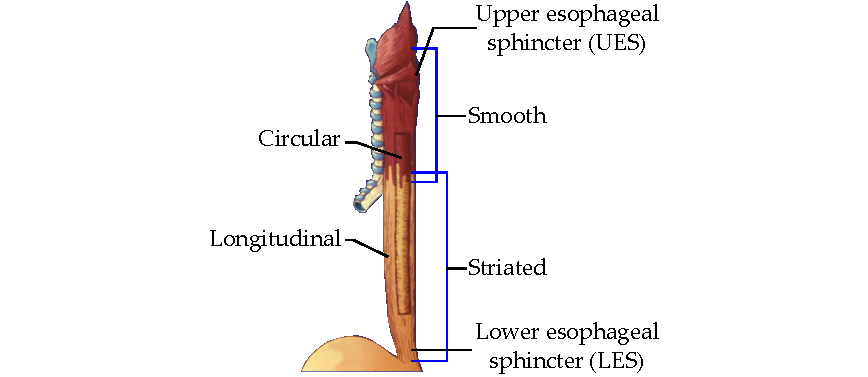
\includegraphics[width=\linewidth]{images/Ch2/fig3_EsophagusMuscle}} \quad
	\caption[Muscular anatomy of esophagus]{Muscular anatomy of esophagus. \citep{mashimo2006physiology}}\label{fig3_EsophagusMuscle}
\end{figure}

\begin{itemize}
	\item Primary peristalsis
	
	\ac{PP} is a voluntary contraction that can occur due to the stimulation of the receptive fields in the esophagus. The primary peristalsis mostly takes place in both striated and smooth muscle fibers. In striated muscle fibers, the peristalsis is controlled by the central swallowing program (neural excitation) (\autoref{tab1_esophagus}) \cite{Dodds1989}.
	
	\item Secondary peristalsis
	
	
	\ac{SP} arises whenever there is a bolus remaining in the esophagus in which stimulus to the oesophageal receptive fields initiates the peristalsis. The peristaltic wave can be activated by the distension of any part of the esophagus (\autoref{tab1_esophagus}) \cite{lang2009brain}.
\end{itemize}

Ghosh et al. \cite{ghosh2006physiology} analysed the \ac{ROT} using \ac{HRM} and digital fluoroscopy. During \ac{PPW} propagation, \ac{PILPS} follows the bolus tail and for successful bolus transport it remains higher than \ac{MIBPS} ($t_1$). As soon as \ac{PPW} enters the ROT ($ t_2$), it starts to slow down, and \ac{PILPS} decreases and hence, esophageal muscle squeeze reduces ($ t_2$ to $t_3$). Concurrently, another wave known as the \ac{IW} begins to compensate the \ac{PPW}. As, IW progresses, it occludes the lumen increasingly ($ t_3$ to $t_5 $) and \ac{PILPS} shifts in front of \ac{MIBPS} ($ t_5 $). IW travels until it fully occludes the lumen ($ t_6$ to $t_7$), and initiates the beginning of \ac{SPW} ($ t_7 $). Concurrently, the \ac{PPW} ends and birth of a new bolus tail takes place. Since for a successful bolus transport, \ac{PILPS} must be higher than \ac{MIBPS}; thus  \ac{MIBPS} jumps ($ t_7$ to $t_8 $). 

\begin{figure}[bth]
	\myfloatalign
	{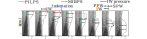
\includegraphics[width=\linewidth]{images/Ch2/fig5_ROT}} \quad
	\caption[Pressure signature and bolus coordination during bolus transport through the Region of Transition (ROT) in a normal subject.]{Pressure signature and bolus coordination during bolus transport through the ROT in a normal subject. \citep{ghosh2006physiology}}\label{fig5_ROT}
\end{figure}

\autoref{tab1_peristalsis} summarizes the effect of different bolus types and bolus volume on the \ac{PILPS}, \ac{MIBPS}, and \ac{BIBPS}. 
\newgeometry{margin=1mm} % modify this if you need even more space
\begin{landscape}
	{\footnotesize
		\vspace*{\fill}
		\vspace*{\fill}
		\vspace*{\fill}
		\begin{longtable}{llllllllll} 
		\caption{Effect of different bolus types and bolus volume on the pressure signature generated by peristaltic waves.}\label{tab1_peristalsis}\\\toprule
Characteristics                                                                                                                                                                                                                    & Bolus attributes                                                                       & \multicolumn{3}{c}{\begin{tabular}[c]{@{}c@{}}Pressure amplitude\\ (mmHg)\end{tabular}}                                               & \begin{tabular}[c]{@{}c@{}}Mean velocity\\ (mms$-1$)\end{tabular} & Ref.      \\
\midrule
&                                                                                    & Upper                                                     & Middle (ROT)                                          & Lower    &                                                           &          \\
\midrule


\multirow{4}{*}{\begin{tabular}[c]{@{}l@{}}The act of swallowing can initiate peristalsis. \\ Food bolus volume, and viscosity can regulate peristalsis.\end{tabular}}                                                          & Dry                                                                                &PILPS = 49 $\pm$ 7.5 &PILPS = 70 $\pm$ 10.7 &          &40.85 $\pm$ 3.6 &  \\
& 1 ml                                                                               &PILPS = 61 $\pm$ 7.5       &PILPS = 66 $\pm$ 6.7&          & 33 $\pm$ 1.9          &   \cite{hollis1975effect}       \\
& 20 ml                                                                              &PILPS = 107 $\pm$ 13     &PILPS = 127 $\pm$ 15.7&          &                                                                 &          \\
\midrule

\multirow{3}{*}{\begin{tabular}[c]{@{}l@{}}PILPS - BIBPS $\ge$ 20 mmHg (2.7 KPa).\\ BIBPS independent of manometric location without \ac{AC}.\\ BIBPS increases at distal part with AC.\\ BIBPS increases with volume and viscosity ($\ge$ 10 ml).\end{tabular}} &  10 ml without AC & \multicolumn{3}{c}{--BIBPS = 12--}                                                                                             &       35.85 $\pm$ 2.0                                                          &                        \\
& 20 ml without AC & \multicolumn{3}{c}{--BIBPS = 15--}                                                                                             &     35.85 $\pm$ 2.0                                                            & \cite{ren1993determinants}                          \\
& 10 ml with AC                                                                      &  BIBPS = 12.0                                                      & BIBPS = 12.0                     & BIBPS = 28.0                       &                                                                 &                           \\                                                                   & 20 ml with AC                                                                      &  BIBPS = 15.0                                                      & BIBPS = 15.0                     & BIBPS = 28.0                       &                                                                 &                           \\                                                                                                                                                                &                                                                                    &\\ 
\midrule



\multirow{6}{*}{Dysphagia patients suffering from Achalasia or Chagas disease.}                                                                                                                                                                                                                 & Dry swallow (Normal)                    & PILPS = 78.7                                                      & PILPS = 45                                                    &          &                                                                 &          \\
& Wet swallow (Normal)                   & PILPS = 95.1                                                      & PILPS = 88.3                                                  &          &                                                                 &          \\
& Dry swallow (Achalasia)       & PILPS = 32.4                                                      & PILPS = 46.1                                                  &          &                                                                 &          \cite{dalmazo2010esophageal}\\
& Wet swallow (Achalasia)               & PILPS = 31.4                                                      & PILPS = 38.9                                                  &          &                                                                 &          \\
& Dry swallow (Chagas)                  & PILPS = 63.8                                                      & PILPS = 24.7                                                  &          &                                                                 &          \\
& Wet swallow (Chagas)             & 75.4                                                      & PILPS = 37.2                                                  &          &                                                                 & \\
\midrule


\multirow{3}{*}{\begin{tabular}[c]{@{}l@{}}Mean velocity of the wave increases from upper to distal part of the esophagus.\\ A significant reduction in the rate of pressure was found in the upper esophagus.\end{tabular}}       & Wet swallow                                                                        & \multicolumn{1}{l}{PILPS = 53.4}                          & \multicolumn{1}{l}{PILPS = 35.0}                        & \multicolumn{1}{l}{PILPS = 69.5} & \multicolumn{1}{l}{}                                            & \multicolumn{1}{l}{} \\
&                                                                                    & \multicolumn{1}{l}{}                                      & \multicolumn{1}{l}{}                                  & \multicolumn{1}{l}{}             & \multicolumn{1}{l}{}                                            & \multicolumn{1}{l}{\cite{dalmazo2010esophageal}} \\
&                                                                                    & \multicolumn{1}{l}{}                                      & \multicolumn{1}{l}{}                                  & \multicolumn{1}{l}{}             & \multicolumn{1}{l}{}                                            & \multicolumn{1}{l}{}\\
\midrule


\begin{tabular}[c]{@{}l@{}}Transition from PPW to SPW occurs in the ROT.\\ Spatial jump of PPW to SPW in the ROT.\end{tabular}                                                                                                    & Bolus swallow                                                                      & \multicolumn{1}{l}{}                 & \multicolumn{1}{l}{\begin{tabular}[c]{@{}l@{}}PILPS=46.5 $\pm$ 12.4\\ MIBPS=32.1 $\pm$ 11.9\end{tabular}}           & \multicolumn{1}{l}{}             & \multicolumn{1}{l}{}                                            & \multicolumn{1}{l}{\cite{clouse1996characteristics}}\\\bottomrule
  
	\end{longtable}}
\end{landscape}

\restoregeometry
\thispagestyle{empty} 


The shortcomings of these techniques are X-ray radiation exposure and catheterization (inserting a manometry catheter) that accumulate to the efforts of swallowing and the general health of subjected individuals.[Roy]

\subsection{Neuronal Circuits of Swallowing: Central Pattern Generators (CPGs)}

The esophageal stage of swallowing, although connected to the pharyngeal stage, is following its own distinctly separate neural control. The \ac{PP} occurs deliberately with the stimulation of receptive territories in the oropharyngeal range, while \ac{SP} happens if bolus or a part of the bolus gets stuck in the esophagus in which stimulation to the oesophageal receptive territories begins the peristalsis \cite{Miller1986,Miller1987}. There are many mechanisms to coordinate the esophageal swallowing process, primarily controlled by both brain stem control and external coordination control. The brain stem control is triggered by patterns of neural or declining cortical input. The findings of \cite{Miller1986,Miller1987}, also support the fact that the contraction of the entire esophagus takes place, which includes both the smooth and striated muscle fibers during \ac{PP}. \ac{PP} is associated with the swallowing, and it is centrally controlled by the activation of the motor neurons \cite{Miller1986,Miller1987}.

The brain stem control consists of three parts for controlling the esophageal swallowing, the \ac{CPG}, pre-motor circuitry, and motor neurons \cite{lang2009brain}. Studies in electrophysiology conducted by Jean \cite{Jean2001,jean1972localization} have proved the existence of the timing pattern generator circuits. The events caused by these generators are natural and local in nature, such that the feedback from the periphery does not affect the generation of the patterns because they persist even in paralyzed animals \cite{jean1972localization}. In other words, it can be written that the pattern generators govern the sequence of the motor responses in the esophageal swallowing process.

The microelectrode experiments conducted by Jean \cite{Jean2001}, showed that the swallowing \ac{CPG} includes two major neuron groups. One group is located in the nucleus tractus solitarii of the dorsal medulla and held responsible for pattern generation and their characteristics like time of triggering, shaping and timing of the rhythmic pattern. The second group is in the ventrolateral medulla, which divides the swallowing drive to the different pools of motor neurons included in swallowing.
The threshold that induces the swallowing depends upon many factors like the type of fluids, touch, the pressure exerted by the food bolus, and range of salivation. By having a sensory feedback mechanism, the threshold and intensity of sequential muscle requirement for the peristalsis can be changed \cite{Miller1987}. Inter and intra-form of reflexes also change or adjust the swallowing to consider the alterations in physiologic functions. These alterations combine the deglutitory inhibition, failed swallow, and \ac{SP} \cite{lang2009brain}.

\subsection{Dysphagia}

The primary purpose of the esophagus is to deliver the food from the mouth to the stomach. Complete food bolus transit is referred to as a successful swallow, and it is associated with effective peristalsis. An ineffective peristaltic wave often leads to a residue of food particles left in the esophagus \cite{ren1993determinants}. 

Any esophageal impairment compromises the efficiency of swallowing, is known as dysphagia \cite{Dodds1989}. Severe pathologies, for instance, benign esophageal strictures from various injuries, esophageal cancer, and esophageal perforations, distressing lumen patency explicitly leading to dysphagia. Unaccompanied by comprehensive care, a vicious cycle materializes as malnutrition and dehydration aggravating the dysphagia itself, subsequently increasing morbidity and even mortality \cite{Groher2015}. The standard clinical practices involve evaluation of the etiology of the swallowing deficit using perception studies, and in vivo analysis, followed by intervention strategies for nutritional support \cite{Kuo2012}. Depending upon the severity, the method of maintaining nutrition, varies from oral dietary supplements, texture modified foods, implanting nasogastric feeding tubes, surgical correction, endoscopic dilation of the sphincters, and esophageal stenting \cite{Groher2015,Cichero2017}.


The estimates show that dysphagia affects one-twelfth of the world's population. Different texture modifications on food like chopping, mashing, and pureeing on food are done across the globe so that the swallowing process in dysphagic patients can be improved. Liquids are often thickened to increase the swallowing time \cite{Cichero2017}. It's highly challenging for such patients to chew and swallow food having high Young's modulus. By introducing some modifications to the food, the effort required for swallowing can be significantly reduced, and it can add nutritional value to their daily oral food intake as well. 

Dysphagia patients often suffer from conditions leading to ineffective peristalsis, and hence remaining residue of food particles in the esophagus \cite{Carrier2007Cognitive}.  For a successful swallow, the intraluminal and the intrabolus pressure must overcome the obstruction created by the esophagogastric junction \cite{jeong2014utilizing,ren1993determinants}. It is often seen that wet and bolus swallows comparatively causes the higher strength of contraction waves (higher \ac{PILPS}) in the distal part of the esophagus than dry swallows. This phenomenon is not observed in the subjects suffering from diseases like achalasia and Chagas disease due to the impairment of the oesophageal nervous system abnormalities. Such kind of nervous abnormalities causes alterations in the motility of the esophagus \cite{dalmazo2010esophageal}.

\section{Stretchable and Flexible Sensors}

Sensors made from stretchable materials could be incorporated into soft robots for sensing its different elements. Due to their flexibility and transparency, sensors manufactured from \ac{CNT}, graphene, and \ac{SNT} have gained much significant attention for application in flexible electronics and the field of robotics. Instead of developing new materials, conventional rigid materials such as silicon and allotropes of carbon are engineered to prepare these sensors.  The principle behind the working of these sensors is when the nanotubes are stretched, gaps and islands are formed on the films of these tubes due to fracture and bundle formation take place, which bridges the gap. This allows the nanotubes to act as strain sensors. By employing different manufacturing processes, the properties of the materials can be differed depending on the type of application. High durability, fast response, and low creep are some of the advantages of soft sensors over their rigid counterparts. \ac{CNT} sensors are popular due to their low cost, linearity and chemical stability. The in-plane strain sensors built from \ac{CNT} exhibits a high piezoresistive response \cite{Miao2011Optimization,miao2012modelling}, but extensive use of these sensors makes the nanotubes buckle due to the release of load, and the effect is known as buckling effect which leads to a wavy structure \cite{Shi2016Graphene}. By filling graphene into the nanotubes, voids can improve the strength of nanotubes significantly, and buckling can be prevented while maintaining the transparency of the material. Table 6and Table 7 summarises some of the \ac{CNT}-based sensors, their characteristics, and their application.

\newgeometry{margin=1mm} % modify this if you need even more space
\begin{landscape}
	{\footnotesize
		\vspace*{\fill}
		\vspace*{\fill}
		\vspace*{\fill}
		\begin{longtable}{llllll} 
		\caption{Different stretchable and flexible sensors, their constructions, advantages, and applications.}\label{tab1_peristalsis}\\\toprule
Name&Materials&Methods&Advantages&Applications&Ref.\\ 
\midrule                                              
\multirow{3}{*}{\begin{tabular}[c]{@{}l@{}}\ac{CNT} embroidered \\graphene (CeG)\end{tabular}}& & Hybridized film of \ac{CNT} and graphene&Increases strength at the nanotubes joints.&&\\
&\ac{CNT} graphene& Chemical vapour deposition (CVD) &Prevention of buckling behaviour.& {\begin{tabular}[c]{@{}l@{}}Motion sensing \\applications (\autoref{fig6_Sensors}a).\end{tabular}}&\cite{Shi2016Graphene}\\
&& \ac{PDMS} was used. &Linear and positive resistance change.&&\\
\midrule                                              
\multirow{3}{*}{CNT film strain sensor} & \multirow{3}{*}{\begin{tabular}[c]{@{}l@{}}Single-walled \ac{CNT} \\ (SWCNT) thin films\end{tabular}} & \multirow{3}{*}{\begin{tabular}[c]{@{}l@{}}Individually removed and laid side by side, \\ with a 1 mm overlap, onto \ac{PDMS}\end{tabular}} & High selectivity against twist.                                                                                                                    &  &          \\
&                                                                                                  &                                                                                                                                        & High durability and reproducibility.                                                                                                                               & {\begin{tabular}[c]{@{}l@{}}Human motion \\detection (\autoref{fig6_Sensors}b,c, and e).\end{tabular}} & \cite{Yamada2011Stretchable} \\
&                                                                                                  &                                                                                                                                        & \begin{tabular}[c]{@{}l@{}}The response of the \ac{CNT} strain sensor \\ to the strain is fast, with a low \\overshoot of 3.0 \% and recovery.\end{tabular} &  &\\

\midrule



\multirow{4}{*}{\begin{tabular}[c]{@{}l@{}}Graphene Porous\\ Network (GPN) - PDMS\end{tabular}} & \multirow{4}{*}{\begin{tabular}[c]{@{}l@{}}Nickel,\\ Graphene\end{tabular}} & Graphene growth.        &                                                                                       & Finger motion.          & \multirow{4}{*}{\cite{pang2016flexible}} \\
&                                                                             & \ac{PDMS} infilteration.& Wide pressure sensing range.                                                          & Blood pressure monitor. &                           \\
&                                                                             & Cutting redundant PDMS. & \begin{tabular}[c]{@{}l@{}}Highest sensitivity among\\ graphene sensors.\end{tabular} & Walking state.          &                           \\
&                                                                             & Ni etching.             &                                                                                       & Degree of finger blood. &               \\\midrule





\multirow{3}{*}{\begin{tabular}[c]{@{}l@{}}Dynamically stretchable\\ solid state supercapacitor\\ using graphene woven fabric (GWF)\end{tabular}} & Polyaniline                                                              & Stretching \ac{PDMS}                & \multirow{3}{*}{\begin{tabular}[c]{@{}l@{}}Excellent stretch ability under\\ high strain.\end{tabular}} & Wearable electronics                                                                       & \multirow{3}{*}{{\cite{zang2015dynamically}}} \\
& \multirow{2}{*}{\begin{tabular}[c]{@{}l@{}}Graphene\\ film\end{tabular}} & Transferring GWF on top of it. &                                                                                                          & \multirow{2}{*}{\begin{tabular}[c]{@{}l@{}}Bendable energy \\ storage device\end{tabular}} &                           \\
&                                                                          & Encapsulation by \ac{PDMS}          &                                                                                                          &                                                                                            & \\ 
\midrule                        
\multirow{4}{*}{\begin{tabular}[c]{@{}l@{}}\ac{CNT} filled\\ Ecoflex\\ composite\end{tabular}} & \multirow{4}{*}{\begin{tabular}[c]{@{}l@{}}\ac{CNT}, vulcanized \\silicone rubber \\ (Ecoflex 00-30)\end{tabular}} & \multirow{4}{*}{\begin{tabular}[c]{@{}l@{}}MWNTs-isoprtyl alcohol (IPA) mixture \\prepared and poured on acrylic mold.\\ Ecoflex was poured, degassed, and\\ cured. Ecoflex penetrated the pourous \ac{CNT}.\end{tabular}} & \multirow{2}{*}{\begin{tabular}[c]{@{}l@{}}Linearity observed between applied strain \\ and resistance change.\end{tabular}} & \multirow{4}{*}{\begin{tabular}[c]{@{}l@{}}Conduit deformation\\ in RoSE\end{tabular}} & \multirow{4}{*}{{\cite{Zhu2016Nanocomposite}}} \\
&                                                                                                                  &                                                                                                                                                                                         &                                                                                                                                 &                                                                                        &                           \\
&                                                                                                                  &                                                                                                                                                                                         & \multirow{2}{*}{\begin{tabular}[c]{@{}l@{}}Wide strain sensing range.\end{tabular}}                                           &                                                                                        &                           \\
&                                                                                                                  &                                                                                                                                                                                         &                                                                                                                                 &                                                                                        &                          
\\\bottomrule
  
	\end{longtable}}
\end{landscape}

\restoregeometry
\thispagestyle{empty} 

\begin{figure}[bth]
	\myfloatalign
	{\includegraphics[width=\linewidth]{images/Ch2/fig6_Sensors}} \quad
	\caption[Various stretchable and flexible sensors.]{Various stretchable and flexible sensors. (a) CeG motion sensing application \cite{Shi2016Graphene}. (b) Image of a bandage strain sensor pasted on the throat for phonation \cite{Yamada2011Stretchable}. (c) Strain sensors fixed to data glove \cite{Yamada2011Stretchable}. (d) Bending of a GPN-PDMS composite \cite{pang2016flexible}. (e) A strain sensor fixed to a stocking for knee motion \cite{Yamada2011Stretchable}. (f) An embedded stretchable sensor for measuring the conduit deformation of RoSE \cite{Zhu2016Nanocomposite}.}\label{fig6_Sensors}
\end{figure}

\newgeometry{margin=1mm} % modify this if you need even more space
\begin{landscape}
	{\footnotesize
		\vspace*{\fill}
		\vspace*{\fill}
		\vspace*{\fill}
		\begin{longtable}{lccccll} 
		\caption{Different stretchable and flexible sensors and their quantitative and qualitative characteristics.}\label{tab1_peristalsis}\\\toprule
Sensor name&Pressure range (KPa)&Strain (\%)&Gauge factor &Thickness&Qualitative characteristics&Ref.\\ 
\midrule                                              
\ac{CeG}                                                        &      & 0 - 20 & 0.36  &      & High linearity and reproducibility.                                                                                          & \cite{Shi2016Graphene}\\
%\midrule
%\begin{tabular}[c]{@{}l@{}}Skin-like pressure and strain sensors\end{tabular} & 1000 & 0 - 50 & 0.004 & 2 mm & \begin{tabular}[c]{@{}l@{}}Can distinguish between pressure and strain.\\Less crosstalk, high transparency.\end{tabular} & \cite{}  \\
\midrule
\begin{tabular}[c]{@{}l@{}}\ac{CNT} film strain sensor\end{tabular} &  & \begin{tabular}[c]{@{}l@{}}0 - 40, \\ 60 - 200\end{tabular} & 0.82, 0.06 &  & \begin{tabular}[c]{@{}l@{}}Fast response, high strain sustainability\\up to 280 \%, high durability (1000 cycles),\\reproducibility, almost temperature independent.\end{tabular} & \cite{Yamada2011Stretchable}   \\
\midrule
\begin{tabular}[c]{@{}l@{}}\ac{GPN}-\ac{PDMS}\end{tabular} & 1000 &\begin{tabular}[c]{@{}l@{}}0 - 18, \\ 22 - 40\end{tabular} & 2.6, 0.85 & 2 mm & & \cite{pang2016flexible}  \\ 
\midrule   
\begin{tabular}[c]{@{}l@{}}\ac{CNT} filled Ecoflex composite\end{tabular} & 140 &0 - 450& 1.2 & 50 $\mu$m &Thin, high strain sustainability. & \cite{Zhu2016Nanocomposite}  \\                                                                             
\bottomrule
  
	\end{longtable}}

\end{landscape}

\restoregeometry
\thispagestyle{empty} 

\section{Biologically inspired control: Central Pattern Generators (CPGs)}

Humans and animals can deliver various rhythmic movements (running, crawling, walking) and processes (swallowing, breathing), which can be done without the involvement of the brain \cite{ijspeert2008central}. Hence, they are known as unsupervised movements, and they are controlled and produced by \ac{CPG}s. \ac{CPG}s are neural systems equipped for creating facilitated patterns of rhythmic movement without any rhythmic inputs from sensory feedback or higher control centers \cite{ijspeert2008central,haghpanah2016generating,fang2016cpg}. Experiments have shown the fact that \ac{CPG} is distributed networks composed of oscillators. Lamprey and salamanders have been observed to have small sections in the spinal column, which are capable of generating rhythmic patterns \cite{delvovlve1999fictive}. Although the \ac{CPG} can produce patterns without any feedback, the sensory feedback plays a significant role in characterizing the trends \cite{mcclellan1993mechanosensory,sigvardt1996effects,kopell1998chains,Miller1987,lang2009brain}. Swallowing, breathing, and gait and its transitions are the areas where clear evidence of CPG control and effect of sensory feedback on it can be seen. Some of the advantages of \ac{CPG} control are, a) fast coordination and short feedback, b) the control signals do not need to know the type of muscle activity involved, and by modulating the signals, the rate of activity can be controlled, and c) providing a low-level distributed control mechanism.
Various methodologies can design the \ac{CPG}s, but before constructing a model of the \ac{CPG}, the following points should be kept in mind \cite{ijspeert2008central}:
\begin{itemize}
	\item The architecture of the \ac{CPG} network must be pre-determined, which includes the number of neurons or oscillators.
	\item The network topology must define the type of couplings to be employed during the coordination among the neurons and oscillators.
	\item The shape of the waveform.
	\item The parameters, their effect on the form of the waveform and how the parameters can influence the characteristics of the waveform.
	\item The effect of the feedback and how the feedback will vary the trajectories.
\end{itemize}

Some of the approaches by which a \ac{CPG} network can be implemented are hand-coding, dynamical system design, and learning and optimization algorithm. The theory of dynamical system can become a strong tool for developing CPG networks. The theory can define the coupling weights and \ac{CPG} parameters, and it can identify the timing of synchronization among the coupled oscillators. Inspiring from the rhythmic biological \ac{CPG}s, many mathematical models of artificial \ac{CPG}s were developed by the researchers so that the \ac{CPG}s can provide the desired rhythmic patterns for different locomotion forms in animals \cite{ijspeert2008central,iwasaki2006analysis,righetti2006dynamic}. Although, it is a powerful tool to set a \ac{CPG} network if the network consists of a small number of neurons and oscillators. If the numbers are large and (or) if the amplitude and frequency of the oscillations cannot be explicitly defined, then applying dynamical theory becomes a rigorous work \cite{fang2016cpg,kim2009central}. In such cases, learning and optimization algorithms can be used in several ways. The approach can be subdivided into two groups: \ac{SL} and \ac{UL} learning. To apply \ac{SL} algorithms, a set of patterns must be present beforehand so that an explicit error function can be defined and minimized to get the desired set of patterns \cite{fang2016cpg,nakanishi2004learning}. Such techniques are limited to circumstances where suitable patterns are available. If the desired patterns are not available, then programmable \ac{CPG}s can be designed by implementing \ac{UL} algorithms \cite{righetti2006dynamic,ijspeert2004simple}.
Numerous scientists created mathematical \ac{CPG} models to produce movement in several robots. Some of the inherent advantages of such biological inspired networks are to ensure consistent motion generation, adaptiveness, robustness, stability, and ability to manipulate its parameters online for different obstacles. Matsuoka \cite{matsuoka1985sustained}, Multivariable Harmonic balance (MHB) \cite{iwasaki2006analysis,iwasaki2008multivariable}, Van-der-pol \cite{righetti2006dynamic}, Hopf \cite{wang2017cpg}, and Rayleigh, are the oscillators used in generating rhythmic patterns in robotics control.

\section{Machine Learning}

The issue of searching for patterns in experimentally collected data is a key one and has a long and efficient history. For example, the broad astronomical observations of Tycho Brahe in the sixteenth century permitted Johannes Kepler to find the experimental laws of planetary motion. Similarly, in the 20th century, the disclosure of regularities in the spectra of atomic structure played a vital part in the improvement and validation of quantum physics. The primary objective in the field of pattern recognition is to discover the regularities in the data automatically by using computer algorithms and then to classify or to regress a set of new data by using these detected regularities. One of the most simple examples for the regression of data is polynomial curve fitting \cite{motulsky1987fitting}. Some of the widespread applications of  \ac{ML} techniques are data mining \cite{kotsiantis2007supervised}, face recognition \cite{Osuna1997Training}, speech recognition, image processing and classification, weather forecasting and system identification \cite{bhattacharya2015relevance,Bongard2007automated}.

Due to the evolution of internet technology, computers, and VLSI, research on \ac{ML} has widened, and its sole objective is to make computers learn by developing different algorithms and techniques \cite{bhattacharya2015relevance}. For instance, an \ac{ML} trained system can distinguish emails based on spam or non-spam emails. There are mainly two parts involved in \ac{ML}, the first one is the representation (training), and the second one is the generalization. The evaluation of the data and the function in some instances is referred to as representation, while in generalization, the performance of the system is checked by introducing an unknown dataset to the network. 

\subsection{Supervised Learning}

All the \ac{ML} techniques can be classified into two types: Supervised Learning (\ac{SL}) and Unsupervised Learning (\ac{UL}) \cite{bhattacharya2015relevance,haykin1994neural}. \ac{SL} is also known as learning with a teacher (\autoref{fig7_SL}). The teacher here represents the knowledge of the environment regarding a set of input and output examples \cite{kotsiantis2007supervised,tipping2001sparse}. The network of interest here does not have any knowledge about the environment. The first step of \ac{SL} is to expose both the teacher and the network to a training vector (set of examples) taken from the environment. The teacher will then be able to provide the desired response for that training vector to the network as it already has that built-in knowledge. The desired response is the optimum action that needs to be performed by the network. The network learns the pattern by varying its parameters with the combined effect of the error signal and the training vector. The adjustment to the parameters is carried out iteratively to emulate the teacher by the network so that the knowledge of the environment can be transferred fully. Finally, the moment at which the training process is complete, the network can deal with the environment solely by itself. The emulation done here is assumed to be optimal in a statistical sense, and the type of \ac{SL} used is known as error-correction learning. The objective of \ac{SL} is achieved by defining a cost function and then by minimizing it over the network parameters. The cost function is taken as an error function regarding the desired response and the actual response with a regularising term for controlling the value of the parameters. The minimum point of the cost function is the desired value for the network parameters at which the network will be able to generate the accurate response for an unknown dataset drawn from the environment, provided the network has been generalized well. One way to think about an \ac{SL} machine is a device that explores a hypothesis space (set of candidate output probable function). \ac{SL} is a set of functions that comprises the hypothesis space and finding out a function from the hypothesis space, which is most likely given an example.  The algorithms used to minimize the cost functions are known as optimization algorithms. In \ac{UL}, there is no involvement of the teacher in supervising the learning process.

 \begin{figure}[bth]
 	\myfloatalign
 	{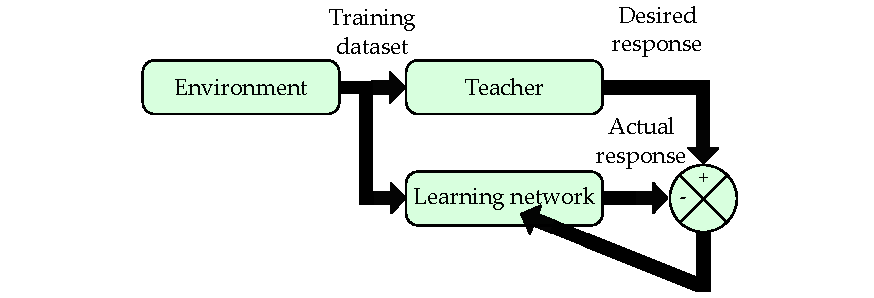
\includegraphics[width=\linewidth]{images/Ch2/fig7_SL2}} \quad
 	\caption[Block diagram of Supervised Learning (SL) with error-correction learning rule.]{Block diagram of Supervised Learning (SL) with error-correction learning rule.}\label{fig7_SL}
 \end{figure}
\subsection{System Identification}

One of the biggest applications of \ac{ML} is \ac{SI} of complex nonlinear dynamical systems whose dynamics cannot be represented by any mathematical model. \ac{SI} is deducing a mathematical description (a model) of a complex nonlinear dynamic system from a series of experimental measurements on the system. The motive for finding out the mathematical description of the dynamic systems are several. Some of them are the detection of faults, system simulation, the prediction for unknown input, and design of the control system. Often, \ac{SI} techniques are reliable when applying the laws of science becomes difficult for building a model. Depending upon the insight knowledge about the system, SI can be categorized into three types \cite{ljung1999system}:

\begin{itemize}
	\item Black-box modeling: \ac{SI} is fully based on the experimentally measured data, and no or minuscule knowledge about the dynamics of the system is available.
	\item Gray-box modeling: A certain degree of insight into the physical system is available, and it is used for the enhancement of empirical modeling.
	\item White-box modeling: Modelling a system by using its physical dynamics comes under the category of white-box modeling.
\end{itemize}

One of the biggest challenges in the field of complex nonlinear dynamical systems is finding out the underlying differential equations (partial) governing the system. The task here is to find out the DE of an unknown system from the observations made during the experiments. The data recorded during the experiments are in a time-series format so that a dynamical model can be built. Many different methods are discussed and proposed in the literature to achieve the required objective for the task. One of the methods for determining the \ac{DE} is \ac{ASR} \cite{Bongard2007automated, schmidt2009Distilling}. The main purpose of \ac{ASR} is to generate symbolic equations from time-series data of a nonlinear dynamic system \cite{Bongard2007automated}. \autoref{ddd}

\begin{equation}
\label{ddd}
{{y}^{(i)}}={{\mathbf{x}}^{(i)}}+{{\varepsilon }^{(i)}}
\end{equation}



\begin{align}
\label{GalerkinProj2}
\begin{split}
{{\mathbf x}(t)}\approx{\mathbf{\tilde{x}}}(t)={\mathbf\Psi}_{r}{\mathbf\Psi}_{r}^{T}{\mathbf{x}}(t)
\end{split}
\end{align}

%\addtocontents{toc}{\protect\clearpage} % <--- just debug stuff, ignore
\ctparttext{
The question arose that this body is the name of one continuous stream of matter — every moment we are adding material to it, and every moment material is being thrown oft by it — like a river continually flowing, vast masses of water always changing places; yet all the same, we take up the whole thing in imagination, and call it the same river. What do we call the river? Every moment the water is changing, the shore is changing, every moment the environment is changing, what is the river then? It is the name of this series of changes. So with the mind.
\begin{flushright}
--\textbf{Swamy Vivekananda}\\
THE VEDANTA\\
(Delivered at Lahore on 12th November, 1897)

\end{flushright}
}
\part{Impermanence}
%\addtocontents{toc}{\protect\clearpage} % <--- just debug stuff, ignor
%%************************************************
\chapter{Literature Review}\label{ch:litreview} % $\mathbb{ZNR}$
%************************************************
%\section{Introduction}

Researchers have developed many soft actuators, sensors and robots that have possible applications in biomedical surgery[2, 3], rehabilitation[4, 5], biomimicking biological processes [6] and research in this area have shown flexibility, agility as well as sensitivity. Some of the advantages of soft robots are: safe human–robot cooperation, minimal effort production,[7, 8] and basic manufacture with negligible coordination[8].

Chapter \ref{ch:introduction} concluded that... 
%*****************************************
%*****************************************
%*****************************************
%*****************************************
%*****************************************

%%************************************************
\chapter{Chapter four}\label{ch:4} % $\mathbb{ZNR}$
%************************************************



%*****************************************
%*****************************************
%*****************************************
%*****************************************
%*****************************************

%%************************************************
\chapter{Chapter five}\label{ch:method} % $\mathbb{ZNR}$
%************************************************


%*****************************************
%*****************************************
%*****************************************
%*****************************************
%*****************************************

%%************************************************
\chapter{Case studies}\label{ch:casestudy} % $\mathbb{ZNR}$
%************************************************
The previous chapter presented the... 
%%************************************************
\chapter{Evaluation}\label{ch:evaluation} % $\mathbb{ZNR}$
This chapter provides an evaluation of the work presented in this dissertation. It aims to examine whether...


%*****************************************
%*****************************************
%*****************************************
%*****************************************
%*****************************************

%%************************************************
\chapter{Conclusions}\label{ch:conclusion} % $\mathbb{ZNR}$
%************************************************
This chapter concludes the thesis by revisiting the research questions raised in Chapter \ref{ch:introduction}...


%*****************************************
%*****************************************
%*****************************************
%*****************************************
%*****************************************


%\include{multiToC} % <--- just debug stuff, ignore for your documents
% ********************************************************************
% Backmatter
%*******************************************************
\appendix
%\renewcommand{\thechapter}{\alph{chapter}}
\cleardoublepage
%\part{Appendix}
%%********************************************************************
% Appendix
%*******************************************************
% If problems with the headers: get headings in appendix etc. right
%\markboth{\spacedlowsmallcaps{Appendix}}{\spacedlowsmallcaps{Appendix}}
\chapter{Appendix A}
%
%%********************************************************************
% Appendix
%*******************************************************
% If problems with the headers: get headings in appendix etc. right
%\markboth{\spacedlowsmallcaps{Appendix}}{\spacedlowsmallcaps{Appendix}}
\chapter{Appendix B}

%%********************************************************************
% Appendix
%*******************************************************
% If problems with the headers: get headings in appendix etc. right
%\markboth{\spacedlowsmallcaps{Appendix}}{\spacedlowsmallcaps{Appendix}}
\chapter{Appendix C}
%%********************************************************************
% Appendix
%*******************************************************
% If problems with the headers: get headings in appendix etc. right
%\markboth{\spacedlowsmallcaps{Appendix}}{\spacedlowsmallcaps{Appendix}}
\chapter{Appendix D}


%********************************************************************
% Other Stuff in the Back
%*******************************************************
\cleardoublepage%********************************************************************
% Bibliography
%*******************************************************
% work-around to have small caps also here in the headline
% https://tex.stackexchange.com/questions/188126/wrong-header-in-bibliography-classicthesis
% Thanks to Enrico Gregorio
\defbibheading{bibintoc}[\bibname]{%
  \phantomsection
  \manualmark
  \markboth{\spacedlowsmallcaps{#1}}{\spacedlowsmallcaps{#1}}%
  \addtocontents{toc}{\protect\vspace{\beforebibskip}}%
  \addcontentsline{toc}{chapter}{\tocEntry{#1}}%
  \chapter*{#1}%
}
%\footnotesize
\printbibliography[heading=bibintoc]

% Old version, will be removed later
% work-around to have small caps also here in the headline
%\manualmark
%\markboth{\spacedlowsmallcaps{\bibname}}{\spacedlowsmallcaps{\bibname}} % work-around to have small caps also
%\phantomsection
%\refstepcounter{dummy}
%\addtocontents{toc}{\protect\vspace{\beforebibskip}} % to have the bib a bit from the rest in the toc
%\addcontentsline{toc}{chapter}{\tocEntry{\bibname}}
%\label{app:bibliography}
%\printbibliography


%\cleardoublepage\pagestyle{empty}

\hfill

\vfill


\pdfbookmark[0]{Colophon}{colophon}
\section*{Colophon}
This document was typeset using the typographical look-and-feel \texttt{classicthesis} developed by Andr\'e Miede and Ivo Pletikosić.
The style was inspired by Robert Bringhurst's seminal book on typography ``\emph{The Elements of Typographic Style}''.
\texttt{classicthesis} is available for both \LaTeX\ and \mLyX:
\begin{center}
\url{https://bitbucket.org/amiede/classicthesis/}
\end{center}
Happy users of \texttt{classicthesis} usually send a real postcard to the author, a collection of postcards received so far is featured here:
\begin{center}
\url{http://postcards.miede.de/}
\end{center}
Thank you very much for your feedback and contribution.

\bigskip

\noindent\finalVersionString

%Hermann Zapf's \emph{Palatino} and \emph{Euler} type faces (Type~1 PostScript fonts \emph{URW
%Palladio L} and \emph{FPL}) are used. The ``typewriter'' text is typeset in \emph{Bera Mono},
%originally developed by Bitstream, Inc. as ``Bitstream Vera''. (Type~1 PostScript fonts were made
%available by Malte Rosenau and
%Ulrich Dirr.)

%\paragraph{note:} The custom size of the textblock was calculated
%using the directions given by Mr. Bringhurst (pages 26--29 and
%175/176). 10~pt Palatino needs  133.21~pt for the string
%``abcdefghijklmnopqrstuvwxyz''. This yields a good line length between
%24--26~pc (288--312~pt). Using a ``\emph{double square textblock}''
%with a 1:2 ratio this results in a textblock of 312:624~pt (which
%includes the headline in this design). A good alternative would be the
%``\emph{golden section textblock}'' with a ratio of 1:1.62, here
%312:505.44~pt. For comparison, \texttt{DIV9} of the \texttt{typearea}
%package results in a line length of 389~pt (32.4~pc), which is by far
%too long. However, this information will only be of interest for
%hardcore pseudo-typographers like me.%
%
%To make your own calculations, use the following commands and look up
%the corresponding lengths in the book:
%\begin{verbatim}
%    \settowidth{\abcd}{abcdefghijklmnopqrstuvwxyz}
%    \the\abcd\ % prints the value of the length
%\end{verbatim}
%Please see the file \texttt{classicthesis.sty} for some precalculated
%values for Palatino and Minion.
%
%    \settowidth{\abcd}{abcdefghijklmnopqrstuvwxyz}
%    \the\abcd\ % prints the value of the length

% ********************************************************************
% Game Over: Restore, Restart, or Quit?
%*******************************************************
\end{document}
% ********************************************************************
